\documentclass[10pt,a4paper]{article}
\usepackage[a4paper,bindingoffset=0.3in,%
            left=0.7in,right=0.7in,top=0.7in,bottom=0.7in,%
            footskip=.125in]{geometry}
\usepackage{multirow}
\usepackage{blindtext}
\usepackage[dvips]{graphics}
\usepackage[dvips]{graphicx}
\usepackage[dvips]{color}
\usepackage{amssymb,latexsym}
\usepackage{rotating}
\usepackage{lscape}
\usepackage{enumerate}
\usepackage{array}

\bibliographystyle{unsrt}

\newcommand{\text}[1]{\textrm{\tiny{#1}}}

\title{The openMMF library: an open source software for multimode driven quantum systems \\ User manual \\ V0.5}
%\author{G. A. Sinuco-Le\'on  \\ \small{\textit{Department of Physics and Astronomy, University of Sussex,Brighton, BN1 9QH, UK}}} 
\date{\today.}

\begin{document}
\maketitle
\tableofcontents

\section{How to build the library and compile the examples}

The openMMF source code includes a \verb Makefile file for compiling and building the library. The user must ensure that \verb make.inc  sets correctly the system's path to the LAPACK and (optionally) the MKL-intel libraries and linking/compiling options. 

When the paths are set correctly, compiling the library requires invoking a single \verb make  command, which will build the library. To indicate whether the MKL library can be used, the user should indicate so in \verb make.inc  . The \verb make  builing options are:

\begin{itemize}
\item \verb make            :  Compiles the library and selected Fortran and C++ examples 
\item \verb make  \verb lib :  compiles the library including support for sparse matrices. This option requires the LAPACK and MKL-intel libraries.
\item \verb make  \verb lib_lapack : compiles the library without support for sparse matrices. This option requires LAPACK.
\item \verb make  \verb Examples_lib : compilies examples under the folder \verb examples/FORTRAN , which uses LAPACK
\item \verb make  \verb Examples_lib_sp : compilies examples under the folder \verb examples/FORTRAN , which uses the MKL library
\item \verb make  \verb Examples_lib_c : compilies examples under the folder \verb examples/CPP  , which uses LAPACK
\item \verb make  \verb Examples_lib_c_sp : compilies examples under the folder \verb examples/CPP , which uses the MKL library
\item \verb make  : run the options \verb lib   and \verb all_examples .
\end{itemize} 
All options of the \verb make   command produces static and dynamical libraries \verb libopenmmf.a  and \verb libopenmmf.so  in the folder \verb ~/lib . A number of \verb .mod  files produced with the building process are moved to the folder \verb ~/include   and they are required for running the  application.

The examples that only require the support of the LAPACK library are compiled with:
\begin{verbatim}
gfortran -o out SourceCode.f90 -I$(INCLUDE_OPENMMF) -L$(LIB_OPENMMF) -lopenmmf $(GFFLAGS)
g++      -o out SourceCode.cpp -I$(INCLUDE_OPENMMF) -L$(LIB_OPENMMF) -lopenmmf -lgfortran $(GFFLAGS)
\end{verbatim}
while code that requires support from the MKL library is compiled by:
\begin{verbatim}
gfortran -o out SourceCode.f90 -I$(INCLUDE_OPENMMF) -L$(LIB_OPENMMF) -lopenmmf 
                               -L$(MKLLIBS) -I$(MKLINC) $(MKLFLAGS)
g++      -o out SourceCode.cpp -I$(INCLUDE_OPENMMF) -L$(LIB_OPENMMF) -lopenmmf -lgfortran
                               -L$(MKLLIBS) -I$(MKLINC) $(MKLFLAGS)
\end{verbatim}


The variables \verb MKLLIBS  , \verb MKLINC  , \verb GFFLAGS  ,   and \verb MKLFLAGS  are defined in the file \verb Makefile . The environmental variables  \verb INCLUDE_OPENMMF   and  \verb LIB_OPENMMF   indicate the paths to the  include and library directories  of the openMMF library. Compilation of \verb C++   source code follows the same formula, using the additional flag \verb -lgfortran   and the corresponding compiler \verb g++ . For an explicit example of usage in this case see the building script under \verb examples/CPP/Makefile .

When running  applications, the environmental variable \verb LD_LIBRARY_PATH   must indicate the path to such a library, which can be done with the shell command:
\begin{verbatim}
export LD_LIBRARY_PATH="/opt/intel/compilers_and_libraries/linux/mkl/lib/intel64:./lib"  
\end{verbatim}
which assumes default folder location of the MKL library and that \verb libopenmmf  is located in \verb ./lib  .


\section{What does the library calculate and how? }
The library can be used to calculate the time-evolution operator, $U(t',t), ~ t'>t$, of systems whose Hamiltonian has the form:
\begin{equation}
H = \sum_{i,j}^D E_{i,j} \left| i\right\rangle \left\langle j \right| + \sum_{i,j}^D \sum_{\ell=1}^N \sum_{n \in Z} V_{i,j}^{\ell,n} e^{i n \omega_\ell t} \left| i\right\rangle \left\langle j \right| + \textrm{h.c.}
\label{eq:Hamiltonian}
\end{equation}
where $D$ is the dimension of the Hilbert space, ${E_{i,j}}$ defines a static component of $H$, $V_{i,j}^{\ell,n}$ is the coupling between the states $i$ and $j$ oscillating at frequency $n \omega_{\ell}$ (i.e. the $n$-th harmonic of the $\ell$-th fundamental frequency $\omega_{\ell}$) and $N$ is the number of incommensurate frequencies.

To calculate the time-evolution operator we generalise the Rotating (or Resonant) Wave Approximation (RWA), taking into account the complex time dependence of Eq. (\ref{eq:Hamiltonian}). For this, we rephrase the problem in terms of building a time-dependent unitary transformation, $U_F(t)$ to a new basis $\{\left| \bar{i} \right\rangle\}$, that leads to a \textit{time-independent} and diagonal Hamiltonian, $\bar{H}$. The operator $U_F(t)$ is called the \textit{micromotion operator} and the new basis is a generalised multimode definition of the \textit{dressed basis}. After applying the standard quantum-mechanical transformation rule to the Schr\"odinger equation \cite{chu1985recent,PhysRevA.81.063626}, this condition becomes:
\begin{eqnarray}
 U_F^\dagger(t) \left[ H(t) - i \hbar \partial_t \right] U_F(t)  &=& \sum_{\bar{i}} \bar{E}_{\bar{i}} \left| \bar{i} \right\rangle \left\langle \bar{i} \right|
\label{eq:Hdressed}
\end{eqnarray}
where $\bar{E}_{\bar{i}}$ is the eigen-energy of the dressed state  $\left| \bar{i} \right\rangle$, which is an eigenstate of the static Hamiltonian $\bar{H}$.

Importantly, in the basis of states defined by this transformation the time evolution operator is diagonal and has the form:
\begin{equation}
\bar{U}(t',t) = \sum_{\bar{i}} e^{-i \bar{E}_{\bar{i}} (t'-t)} \left| \bar{i} \right\rangle \left\langle \bar{i} \right|
\label{eq:dressedtimeevolution}
\end{equation}
which let us to calculate the time evolution operator in the original basis $\left\{ \left| i\right\rangle\right\}$, just by inverting the transformation $U_F(t)$, according to \cite{PhysRevA.81.063626}:
\begin{equation}
U(t',t) = U_F(t') \bar{U}(t',t) U_F(t)
\label{eq:baretimeevolution}
\end{equation}

To formulate a fully defined computational problem, we express the unitary transformation $U_F(t)$ as the multifrequency Fourier series \cite{ho1983semiclassical}:
\begin{equation}
U_F(t) = \sum_{\vec{n}} U_{i,\bar{i}}^{\vec{n}} e^{-i\vec{\omega} \cdot \vec{n}t} \left| i \right\rangle \left\langle \bar{i} \right|
\label{eq:micromotionexpansion}
\end{equation}
where $\vec{\omega} = (\omega_1,\omega_2,\ldots,\omega_N)$ and $\vec{n}$ is a $N$-dimensional vector of integers. After plugging this expansion in Eq. (\ref{eq:Hdressed}) and performing an integral over time, we obtain a fully defined eigenproblem for the eigenvalues $\bar{E}_{\bar{i}}$ and Fourier components of the unitary transformation $U_{i,\bar{E}}^{\vec{n}}$:
\begin{equation}
\sum_j(E_{i,j} - \hbar \vec{n} \cdot \vec{\omega})U^{\vec{n}}_{j,\bar{i}} + \sum_{j} \sum_{\vec{m}} \left[ V^{\vec{m}}_{i,j} U^{\vec{n}+\vec{m}}_{j,\bar{i}} + V^{\vec{m}*}_{ji} U^{\vec{m}-\vec{n}}_{j,\bar{i}}\right] = \bar{E}_{\bar{i}}U^{\vec{n}}_{i,\bar{i}}
\label{eq:multimodeeigenproblem}
\end{equation}
where $\vec{n}_{\ell,m} = \vec{n} + m P_{\ell}$ with $P_{\ell} = (0,\ldots, 1, \ldots,0)$ the projector at the $\ell-$th position. To obtain a finite matrix representation of this problem we truncate the sum over the number of modes of the Fourier expansion Eq. (\ref{eq:micromotionexpansion}). 

This formulation to calculate the time-evolution operator is equivalent to the multimode Floquet representation of the Hamiltonian that introduces an extended Hilbert space $\left| E_i,\vec{n} \right\rangle$  \cite{ho1983semiclassical,verdeny2016quasi}. However, the semiclassical description presented here makes emphasis in the physically accessible states. 


\section{Use of the library}

Here we illustrate the use of the library's functionality considering a qubit driven by two harmonic forces.  The Hamiltonian of this system has the form:

\begin{equation}
H = \hbar \omega_0 S_z + \hbar \Omega_1 \cos(\omega_1 t) S_x + \hbar \Omega_{2,x} \cos(\omega_2 t) S_x + \hbar \Omega_{2,y} \cos(\omega_2 t)  S_z
\label{eq:dressedqubitmodel}
\end{equation}
The Fortran and C++ source codes to find the time-evolution operator are in the files:
\begin{itemize}
\item  \verb examples/FORTRAN/main_DressedQubit.f90  .
\item  \verb examples/CPP/main_dressedqubit.cpp  .
\end{itemize}

\subsection{Declaration of the Hamiltonian \label{subsec:init}}

First of all, we should declare the two derived types:
\begin{verbatim}
  TYPE(ATOM)                                       ID
  TYPE(MODE),       DIMENSION(:),   ALLOCATABLE :: FIELDS
\end{verbatim}

\noindent 
The variable \verb ID  contains information about the type of system, such as the number of levels and their energy spectrum (see the declaration of \verb TYPE(ATOM)   in Section \ref{sec:derivedtypes}).  The derived type \verb FIELDS   stores information required to build the components of the Hamiltonian as well as the explicit matrix representation of the couplings.

In this concrete example, the components of \verb ID  are initialised by calling the subroutine:
\begin{verbatim}
  CALL FLOQUETINIT(ID,'qubit',INFO)
\end{verbatim}
The second argument indicates the type of system (here 'qubit'), which, is sufficient to initialise the variable  \verb ID   :
\begin{verbatim}
 ID%id_system = 1 
 ID%D_BARE    = 2 
\end{verbatim}
where \verb ID%D_BARE  indicates the dimension of the Hilbert space.

Additional options of the function \verb FLOQUETINIT   are presented in section \ref{sec:InitOptions}, which are useful for initialising some frequently used physical systems with default parameters. When dealing with a general quantum system (i.e. with an arbitrary energy spectrum), there is no need to call this function and the values of a variable of \verb TYPE(ATOM)  must be initialised explicitly.

In the source code, the next relevant instruction is the definition of an integer vector that provides information about the number of driving frequencies. The integer array \verb MODES_NUM   is allocated with size 3, indicating that the system will be driven by two fundamental frequencies (corresponding to $\ell = 1,2$ in Eq. \ref{eq:Hamiltonian}), since the first component is reserved to the static part of the Hamiltonian. The values of the elements of this array indicate the number of driving harmonics of each frequency, which here we set to $1$ (making $n=1$ in Eq. \ref{eq:Hamiltonian}). 

The total number of driving frequencies is equal to the sum of all elements of the array \verb MODES_NUM . The user then should allocate sufficient memory space to store each one of the matrix representations of the couplings $V^{\ell,n}$. This is done with the sequence of instructions:

\begin{verbatim}
  TOTAL_FREQUENCIES = SUM(MODES_NUM,1)
  ALLOCATE(FIELDS(TOTAL_FREQUENCIES))
  DO m=1,TOTAL_FREQUENCIES
     ALLOCATE(FIELDS(m)%V(ID%D_BARE,ID%D_BARE))
  END DO
\end{verbatim}

By default the first element of the array of \verb FIELDS   is reserved for the static component of the Hamiltonian, which includes the spectrum of the static system as diagonal elements of the matrix \verb FILEDS(1)%V  .  The next step then consist in defining all components of the Hamiltonian. For a quantum system with arbitrary energy spectrum, each one of the matrices \verb FIELDS(m)%V   must be declared explicitly. 

When dealing with spin systems, as in the present example, each component of the Hamiltonian can be written as:
\begin{equation}
V^{\ell,n} = e^{\phi_x} X S_x + e^{\phi_y} Y S_y + e^{\phi_z} Z S_z
\label{eq:Vspinparametrisation}
\end{equation}
where $S_i$ is the angular momentum operator. Therefore, we need only six parameters (three phases and three amplitudes) to define the coupling matrices. 

These six parameters should be declared explicitly for each one of the the driving modes, along with the frequency ( \verb omega  )  and the corresponding number of modes to be included in the Fourier expansion of the evolution operator (\verb N_Floquet ). The values of these parameters are initialised as follows:
\begin{center}
  \begin{tabular}{ |l | c | }
    \hline
    Source code & Parameter in Eq. (\ref{eq:Vspinparametrisation}) \\ \hline
    \verb FIELDS(1)%X=0.0 & $X$ \\ \hline
    \verb FIELDS(1)%Y=0.0 & $Y$ \\ \hline
    \verb FIELDS(1)%Z=1.0 & $Z$ \\ \hline
    \verb FIELDS(1)%phi_x=0.0 & $\phi_z$ \\ \hline
    \verb FIELDS(1)%phi_y=0.0 & $\phi_z$ \\ \hline
    \verb FIELDS(1)%phi_z=0.0 & $\phi_z$ \\ \hline
    \verb FIELDS(1)%omega=0.0 & $\omega$ \\ \hline
    \verb FIELDS(1)%N_Floquet = 0   & $N$ \\ 
    \hline
  \end{tabular}
\end{center}
where we have a direct correspondence with Eq. (\ref{eq:Vspinparametrisation}). This set of instructions is repeated for each one of the driving fields, as can be seen in the source code.

\subsection{Hamiltonian components}

The instructions detailed before let us to build the matrix representation of the terms in Eq. (\ref{eq:Vspinparametrisation}). This is done simply by calling the subroutine:

\begin{verbatim}
CALL  SETHAMILTONIANCOMPONENTS(ID,size(modes_num,1),total_frequencies,MODES_NUM,FIELDS,INFO)
\end{verbatim}
which results in storing the coupling $V^{\ell,n}$ in the set of matrices \verb FIELDS(r)%V , with \verb r=1,total_frequencies .

We remind the user that when the system of interest is not one of the default types defined in section \ref{subsec:init}, the user must define explicitly and in full all the coupling matrices. For an example of this situation, see  the source file  \verb example/FORTRAN/main_lattice.f90 .

\subsection{Multimode Floquet matrix and diagonalisation}

Once the components of the Hamiltonian are defined (i.e the complete set of matrices \verb FIELDS(r)%V   has been initialised), the multimode Hamiltonian can be calculated calling the function:

\begin{verbatim}
  CALL MULTIMODEFLOQUETMATRIX(ID,size(modes_num,1),total_frequencies,MODES_NUM,FIELDS,INFO)          
\end{verbatim}

As a result of this call, the system stores the full multimode Floquet matrix on the left-hand side of Eq. (\ref{eq:multimodeeigenproblem}) in the matrix \verb H_FLOQUET. This matrix is defined in the module \verb ARRAYS   and  can be accessed (and modified!) by all computational routines that include this module. The size of this matrix is calculated internally and stored in the parameter \verb h_floquet_size , which is also a global variable. 

The library includes a subroutine to evaluate a sparse representation of this matrix, which results after invoking:
\begin{verbatim}
  CALL MULTIMODEFLOQUETMATRIX_SP(ID,SIZE(MODES_NUM,1),total_frequencies,
                                 MODES_NUM,FIELDS,VALUES,ROW_INDEX,COLUMN,INFO)
\end{verbatim}
 
Setting INFO = 0, this instruction produces the representation of the Floquet matrix \verb H_FLOQUET   in the three array variation of the Compressed Sparse Row (CSR) storage format. With INFO=6, we get the matrix stored as three arrays of equal length, corresponding to values, rows and columns positions. The non-zero values of the matrix are stored in the complex array \verb VALUES ,  and the information about their location is encoded in the integer arrays \verb COLUMN   and \verb ROW_INDEX . The size of these three arrays are evaluated internally.

The library includes wrappers to diagonalisation subroutines from the Lapack and the MKL-intel (for the sparse CSR representation) libraries. These functions are called using:

\bigskip
\noindent
Lapack :  
\begin{verbatim}
 CALL  LAPACK_FULLEIGENVALUES(U_F,SIZE(H_FLOQUET,1),E_FLOQUET,INFO)
\end{verbatim}

\noindent
MKL:
\begin{verbatim}
 CALL MKLSPARSE_FULLEIGENVALUES(D_MULTIFLOQUET,SIZE(VALUES,1),VALUES,ROW_INDEX,
                                                     COLUMN,E_L,E_R,E_FLOQUET,U_F,INFO)
\end{verbatim}

In both cases, the eigenvalues are stored in the array \verb E_FLOQUET   and the eigenvectors are stored as columns of the matrix \verb U_F. Remember that these eigenvectors correspond to the coefficients of the multimode Fourier decomposition of the micromotion operator Eq. (\ref{eq:micromotionexpansion}). Invoking the MKL subroutine requires two additional parameter \verb E_L  and \verb E_R  : the lower and upper bounds of the interval to be searched for eigenvalues, respectively. The user is responsible to set meaningful values of both parameters. 


The MKL sparse solvers requires the use of the variation of the Compressed sparse row (CSR) representation of the matrix, which is produced by sorting the array of ROW position, in such a way that all non-zero values of a given row become stored consecutively. This sorting is done using a \verb QUICK_SORT  algorithm by Robert Renka (OAK Ridge Natl. Lab, US) accessible from the  Alan Miller's Fortran Software website \cite{MillerSoftware}.  Alternatively, calling the function \verb MULTIMODEFLOQUETMATRIX_SP  with the variable \verb INFO=6  , the user obtains the extended Hamiltonian represented by the three arrays of  \verb value, \verb column, \verb row ,  which can be used with a different eigenvalue solver for sparse matrices.

\subsection{Time-evolution operator}

With the full spectrum of \verb H_FLOQUET , the time evolution operator  between \verb T1  and \verb T2 ,  corresponding to Eq. (\ref{eq:baretimeevolution}), can be evaluated calling the function:
\begin{verbatim}
CALL MULTIMODETIMEEVOLUTINOPERATOR(SIZE(U_F,1),SIZE(MODES_NUM,1),MODES_NUM,U_F,E_FLOQUET,
                                                          ID%D_BARE,FIELDS,T1,T2,U_AUX,INFO)
\end{verbatim}
which produces the matrix representation of the operator in Eq. (\ref{eq:baretimeevolution}).  The time evolution operator is stored in the complex matrix \verb U_AUX , whose size is equal to the number of bare states \verb ID%D_BARE .

\subsection{Micromotion operator}

The micromotion operator is the time-dependent unitary transformation between the bare basis and the basis of state where the Hamiltonian is time-independent. Since we know the Fourier decomposition of this transformation via the diagonalisation of \verb H_FLOQUET , we can evaluate the instantaneous transformation, e.g. at time \verb T1, using the subroutine: 

\begin{verbatim}
 CALL MULTIMODEMICROMOTION(ID,SIZE(U_F,1),NM,MODES_NUM,U_F,E_FLOQUET,ID%D_BARE,
                                                               FIELDS_,T1,U_F1,INFO)
\end{verbatim} 
which produces the matrix representation of the operator in Eq. (\ref{eq:micromotionexpansion}). This micromotion operator is stored in the square matrix \verb U_F1  of size \verb ID%D_BARE .

\subsection{Identifying the dressing modes}

In several applications is useful to define a dressed basis of states and the openMMF library includes functions to simplify the evaluation of the evolution operator in this basis. For this, first the user should identify the subset of driving fields that define the dressed states. This is done using an integer array with as a many components as dressing fields. The elements of this array indicate the indices of the fields corresponding to the array \verb modes_num . For example, if there is only one dressing field and it corresponds to the second component of the array \verb MODES_NUM, then the array that indicates the dressing field, \verb DRESSINFIELDS_INDICES ,  must be:

\begin{verbatim}
INTEGER, DIMENSION(2) :: DRESSINGFIELDS_INDICES
DRESSINGFIELDS_INDICES(1) = 1 ! THE STATIC COMPONEN
DRESSINGFIELDS_INDICES(2) = 2 ! THE FIRST DRIVING FIELD, WHICH DRESSES THE SYSTEM
\end{verbatim} 

With this, the Fourier decomposition of the micromotion operator defining the dressed basis in Eq. (\ref{eq:micromotionexpansion}), can be obtained simply by calling the function:

\begin{verbatim}
 CALL MICROMOTIONFOURIERDRESSEDBASIS(ID,DRESSINGFIELDS_INDICES,MODES_NUM,
                                                     FIELDS,U_FD,E_DRESSED,INFO)
\end{verbatim}
The Fourier components $U_{i,\bar{i}}^{\vec{n}}$ are stored in the matrix \verb U_FD  and the spectrum of dressed energies, $\bar{E}_{\bar{i}}$,  are stored in the array \verb E_DRESSED .  With these two elements, we can calculate the micromotion operator of the dressed basis using the subroutine:

\begin{verbatim}
CALL MICROMOTIONDRESSEDBASIS(ID,MODES_NUM,DRESSINGFIELDS_INDICES,FIELDS,U_FD,
                                                            E_DRESSED,T1,U_FD_1,INFO) 
\end{verbatim}

The micromotion operator at T1 is then stored as the square matrix \verb U_FD_1 . This set of instructions let us to evaluate the time-evolution operator in the dressed basis using the sequence:

\begin{verbatim}
   CALL MICROMOTIONDRESSEDBASIS(ID,MODES_NUM,DRESSINGFIELDS_INDICES,FIELDS,U_FD,
                                                             E_DRESSED,T1,U_F1,INFO) 
   CALL MICROMOTIONDRESSEDBASIS(ID,MODES_NUM,DRESSINGFIELDS_INDICES,FIELDS,U_FD,
                                                             E_DRESSED,T2,U_F2,INFO) 
        
   ! ---- CALCULATE THE TIME-EVOLUTION OPERATOR IN THE DRESSED 
   ! ---- BASIS USING THE PREVIOUSLY CALCULATED IN THE BARE BASIS

   U_AUX = MATMUL(TRANSPOSE(CONJG(U_F2)),MATMUL(U_AUX,U_F1)) 

\end{verbatim}

\section{Typical performance}
The efficiency of the library is limited by the capability to solve the eigenvalue problem of the multimode Floquet Hamiltonian. Fig. \ref{fig:performance}(a) compares the execution times for a single diagonalisation of the Floquet HamiltonianBosonic and Fermionic Hubbard models, as functions of the size of the matrix (red and blue data/lines). The source codes can be found in \verb examples/FORTRAN/MANYBODYHUBBARD/  and the model Hamiltonian are:
\begin{eqnarray}
H_{Bosons}(t)   &=&  (t+ \Delta t \cos(\omega t + \phi))\sum_{<i,j>}   b_i b_j^\dagger  + \frac{u}{2}\sum_j  n_j(n_j-1) \nonumber \\
H_{Fermions}(t) &=&   (t+ \Delta t \cos(\omega t + \phi)) \sum_{i,\sigma} (f_{i,\sigma} f_{i+1,\sigma}^\dagger +  f_{i+1,\sigma}^\dagger f_{i,\sigma})  + u \sum_j n_{j,\uparrow} n_{j,\downarrow} \nonumber 
\end{eqnarray}
and we use the parameters $t=1, u=0.5, \phi = 0.0, \omega = 1.0, \Delta t = 0.2$. To vary the size of the Floquet Hamiltonian we increase the number of Floquet manifolds. 

\begin{figure}
\centering
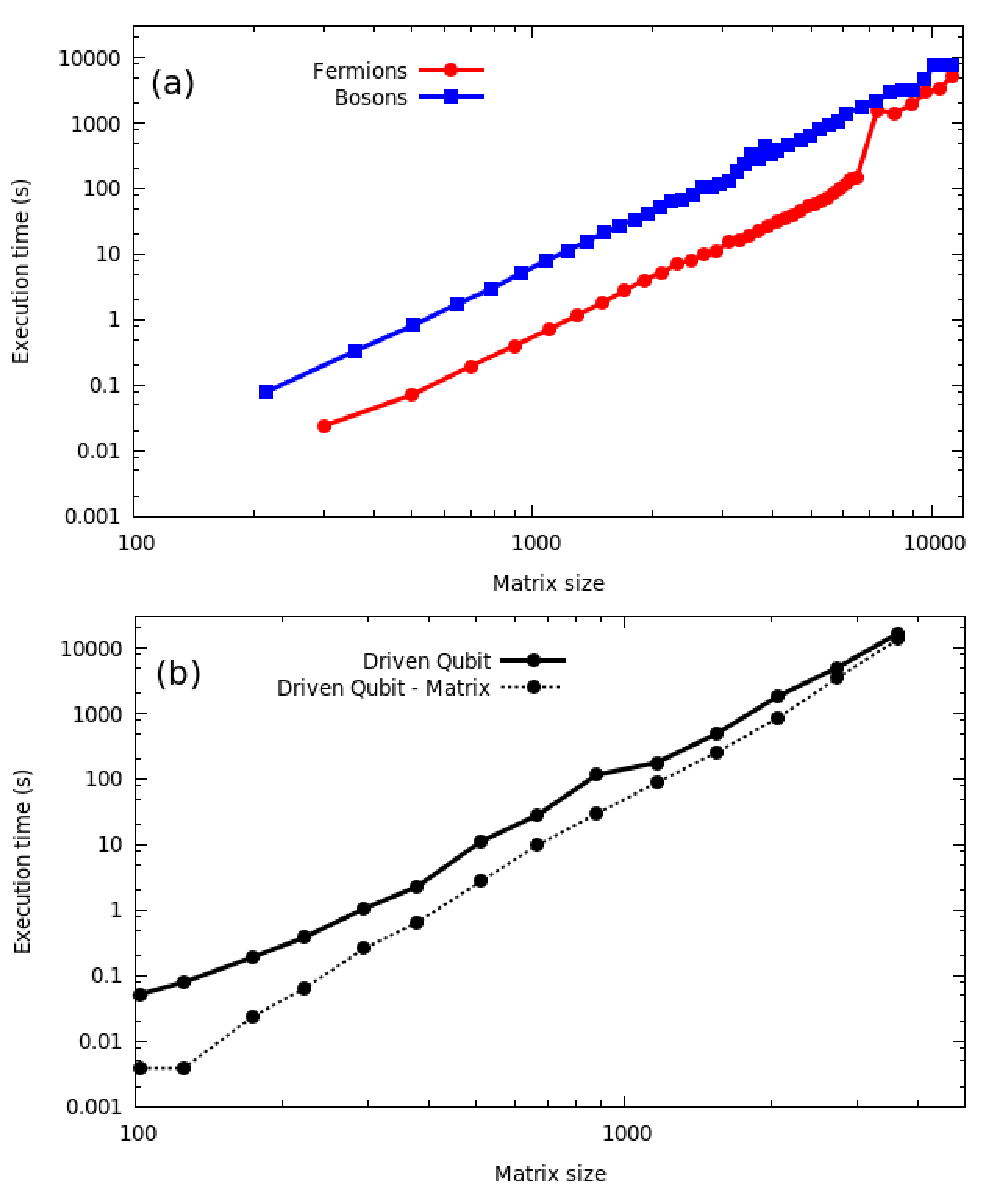
\includegraphics[width=12cm]{openmmf_timing.ps}
\caption{\label{fig:performance} (a) Execution time of a single iteration using OPENMMF. The red data shows results for the Fermionic model with L=5 sites and Nup=1 and Ndown= 2 particles with spin up and down, respectively. In blue, results of the Bosonic model with L=3 sites and N=7 particles. In both cases, the tunnelling and on-site parameters are set to t=1.0 u = 0.5. The driving originates from a harmonic modulation of the tunnelling with amplitude tdriving=0.2 and frequency w= 1.0. We vary the number of Floquet manifolds, which leads to the variation of the matrix size. (b) Execution time to evaluate a single time-step of the evolution of a driven qubit with a band-limited background noise.  The matrix size reflects the number of frequencies contributing to the noisy field. The solid line shows to total execution time. The dashed line shows the execution time to evaluate the Floquet Hamiltonian using the sparse representation. }
\end{figure}

For these tests, the library performs two tasks: evaluates the Floquet Hamiltonian and use LAPACK to obtain the spectrum (only once for each matrix size). The Hamiltonian corresponds to a periodically driven Hubbard model (with near-neighbour tunnelling and on-site interaction) and the matrix dimension is given by the number of Floquet manifolds.

Figure \ref{fig:performance}(b) shows the execution time required to evaluate a single time-step of the time-evolution operator of driven qubit with a noisy background. The Hamiltonian of this system is:
\begin{equation}
H = \hbar \omega_0 S_z + \hbar \Omega S_x \cos (\omega t + \phi) + \sum_\ell^N \Delta_i \cos(\ell \omega/N t + \phi_i)
\end{equation}
with $N$ the number of frequencies contributing to the noisy field, $\Delta_i$ and $\phi_i$ random amplitudes and phases, respectively. With this, the noise frequency is limited up to the driving frequency $\omega$. The matrix size reflects the number of components of the noisy driving. 

In this case we use a DRIVER subroutine and build a sparse representation of the multimode Hamiltonian. In contrast to the previous test, we observe that the matrix building and diagonalisation take about the same fraction of the total time. However, a direct comparison of the total times between these two examples is not straightforward since the structure of the Floquet matrix of the two problems is significantly different. 

These results give us a rough idea of the scaling of the execution time with the matrix size, as well as the possible performance bottlenecks. These tests were performed using a DELL XPS with an Intel Core i7 vPro @ 2.7 GHz and 8GB of RAM. The machine runs on Linux Mint 17.2 Rafaela, with gcc-4.9.4


\section{Default system types}
\label{sec:InitOptions}

The openMMF library defines three different system types by default. These are Qubit, Spin and the ground state of several alkali atoms. A general system with $D$ energy leveles can be defined using the ``spin" type and setting by hand all coupling matrices.  

\subsection{Qubit}
This type represents a two level system, where the couplings with the oscillating field are of the form
\begin{equation}
V^{\ell,n} = X S_x e^{\phi_{\ell,x}} +  Y S_y e^{\phi_{\ell,y}} + Y S_z e^{\phi_{\ell,z}}
\end{equation}
with $S_i, i\in{x,y,z}$ the set of spin $1/2$ angular momentum operators with $\hbar := 1$.

The corresponding derived type is initialised with the instruction: 
\begin{verbatim}
 FLOQUET_INIT(ID,'qubit',INFO)
\end{verbatim}

\subsection{Spin of total angular momentum $S_z$}
This type represents a system with $2 S_z + 1$ equally space energy levels, where the couplings with oscillating fields are of the form:
\begin{equation}
V^{\ell,n} = X S_x e^{\phi_{\ell,x}} +  Y S_y e^{\phi_{\ell,y}} + Y S_z e^{\phi_{\ell,z}}
\end{equation}
with $S_i, i\in{x,y,z}$ the set of  angular momentum operators with total spin $S_z$.

The corresponding derived type is initialised with the instruction:
\begin{verbatim}
 FLOQUET_INIT(ID,'spin',2*Sz,INFO) 
\end{verbatim}
where the third argument is a \verb DOUBLE \verb PRECISION   variable equal to the double of the projection of the total angular momentum.

The matrix representation of the angular momentum operators $s_i$ is build using \cite{sakurai1995modern}:
\begin{eqnarray}
\left\langle S, m'\right| S_x \left| S,m\right\rangle&=& \frac{1}{2} \left[\sqrt{(S-m)(S+m+1)}\delta_{m,m'+1} + \sqrt{(S+m)(S-m+1)}\delta_{m,m'-1} \right]  \label{eq:S_x}\\
\left\langle S, m'\right| S_y \left| S,m\right\rangle&=& \frac{i}{2} \left[\sqrt{(S-m)(S+m+1)}\delta_{m,m'+1} - \sqrt{(S+m)(S-m+1)}\delta_{m,m'-1} \right]  \label{eq:S_y}\\
\left\langle S, m'\right| S_z \left| S,m\right\rangle&=& m\delta_{m,m'} \label{eq:S_z} 
\end{eqnarray}

\subsection{Ground state Alkali atoms.}
The effective model of an alkali atom consist of an electron with zero orbital angular momenta interacting with a static nucleus. These two particles interact via their magnetic moments, which define two manifolds of states corresponding to the total angular momenta $F=I\pm1/2$. The library can be used to study inter and intra manifold dynamics.

\noindent
For example, to study the dynamics with focus on the manifold with total angular momentum $F=I-1/2$ ('L', for lower), the corresponding \verb ID  can be obtained by invoking: 
\begin{verbatim}
CALL FLOQUET_INIT(ID,SPECIE_NAME,'L',INFO) 
\end{verbatim}

and the Hamiltonian components are built assuming the form:
\begin{equation}
V^{\ell,n} = \frac{\mu_B g_{I-1/2} B_x}{A} F_x e^{\phi_{\ell,x}} +  \frac{\mu_B g_{I-1/2} B_y}{A} F_y e^{\phi_{\ell,y}} + \frac{\mu_B g_{I-1/2} B_z}{A} F_z e^{\phi_{\ell,z}}
\end{equation}

Similarly, to study the dynamic of the manifold with $F=I+1/2$ ('U', for upper), the system is initialised using:
\begin{verbatim}
 CALL  FLOQUET_INIT(ID,SPECIE_NAME,'U',INFO) 
\end{verbatim}
which assumes couplings of the form
\begin{equation}
V^{\ell,n} = \frac{\mu_B g_{I+1/2} B_x}{A} F_x e^{\phi_{\ell,x}} +  \frac{\mu_B g_{I+1/2} B_y}{A} F_y e^{\phi_{\ell,y}} + \frac{\mu_B g_{I+1/2} B_z}{A} F_z e^{\phi_{\ell,z}}
\end{equation}

The atomic gyromagnetic factor is defined by:
\begin{equation}
     g_F = g_J*(F*(F+1) - I*(I+1) +J*(J+1))/(2*F*(F+1)) + g_I*(F*(F+1) + I*(I+1) - J*(J+1))/(2*F*(F+1))!
\end{equation}
with $F=I \pm 1/2$.  The matrix representation in each case follows the same procedure as in the case of a spin system. 

Finally, when both manifolds are of interest, we should use:
\begin{verbatim}
CALL FLOQUET_INIT(ID,SPECIE_NAME,'B',INFO) 
\end{verbatim}
which prepares the system to initialise couplings of the form:
\begin{equation}
V^{\ell,n} = \frac{\mu_B  B_x}{A} (g_J J_x + g_I I_x) e^{\phi_{\ell,x}} +  \frac{\mu_B B_y}{A} (g_J J_y + g_I I_y) e^{\phi_{\ell,y}} + \frac{\mu_B B_z}{A} (g_J J_z + g_I I_z) e^{\phi_{\ell,z}}
\end{equation}

In this case, the angular momentum operators are represented in the uncoupled basis $\left| I,J,m_I,m_J \right\rangle$, corresponding to a tensor multiplication of the matrices resulting from Eqs. (\ref{eq:S_x})-(\ref{eq:S_z}) representing $I_i$ and $J_i$.

In all these cases, after invoking the initialisation routine \verb FLOQUET_INIT   and defining the parameters of the couplings using the derived data type \verb TYPE(MODES)::FIELDS, the matrix representation of each component of the Hamiltonian can be obtained with a single call to the subroutine:
\begin{verbatim}
CALL SETHAMILTONIANCOMPONENTS(ID,size(modes_num,1),total_frequencies,MODES_NUM,FIELDS,INFO) 
\end{verbatim}
where \verb total_frequencies   is the total number of driving fields (including a static component). For a complete example see the source code at \verb examples/FORTRAN/main_87Rb.f90 .

\section{List of examples}
\subsection{Python}
Build the examples running \verb make  in the folder \verb examples/PYTHON  .

\begin{tabular}{p{5.5cm}p{9.5cm}}
main\_87Rb.py & Evaluates the time-evolution and spectrum of a driven atom of 87Rb.\\
main\_DressedQubit.py  & Evaluates the time evolution of a dressed qubit in the bare and dressed basis. \\
main\_floquetinit.py  & Illustrates the optional systems.\\
main\_qubit\_driver.py  & Evaluates the tim-evolution operator of a driven qubit using a DRIVER subroutine.\\
main\_qubit.py  & Evaluates the time-evolution operator of a driven qubit.\\
main\_qubit\_sp.py & Evaluatese the time-evolution operator of driven qubit using the sparse representation of the Hamiltonian.\\  
openmmf.py  & Defines the Python wrappers. 
\end{tabular}
\subsection{C++}
Build the examples running \verb make  in the folder \verb examples/CPP  . 

\begin{tabular}{p{5.5cm}p{9.5cm}}
main\_DressedQubit.cpp  & Evaluates the time evolution of a dressed qubit in the bare and dressed basis. \\
main\_DressedQubit\_SP.cpp & Evaluates the time evolution of a dressed qubit in the bare and dressed basis using the sparse representation of the Hamiltonnian. \\
main\_qubit\_driver.cpp & Evaluates the tim-evolution operator of a driven qubit using a DRIVER subroutine.\\
main\_qubit.cpp  & Evaluates the time-evolution operator of a driven qubit.\\
main\_qubit\_sp.cpp & Evaluatese the time-evolution operator of driven qubit using the sparse representation of the Hamiltonian.\\  
MultimodeFloquet.h & Prototype of the C++ wrapper functios. 
\end{tabular}
\subsection{Fortran}
Build the examples running \verb make  in the folder \verb examples/FORTRAN  . 

\begin{tabular}{p{5.5cm}p{9.5cm}}
main\_qubit\_Shirley.f90 & Evaluates the time-evolution operator of a driven qubit with parameters as in the classical paper by Jon Shirley.\\
main\_qubit.f90  & Evaluates the time-evolution operator of a driven qubit.\\
main\_qubit\_SP.f90& Evaluatese the time-evolution operator of driven qubit using the sparse representation of the Hamiltonian.\\  
main\_qubit\_DRIVER.f90 & Evaluates the tim-evolution operator of a driven qubit using a DRIVER subroutine.\\
main\_QuantumInterference.f90 & Evaluates the time-evolution of a bichromatically driven qubit. \\
main\_qubit\_noise\_SP.f90 & Evaluates the time-evolution operator of a driven qubit ina noisy environment. Uses a sparse representation of the Hamiltonian. \\
main\_halfspin\_DRIVER.f90  & Evaluates the time-evolution operator of a two-level system (defined with 'spin') using a DRIVER subroutine, \\
main\_spin\_DRIVER.f90  & Evaluates the time-evolution operator of a L-level system (defined with 'spin') using a DRIVER subroutine, \\
main\_lattice.f90  &  evaluates the spectrum and micromotion of a driven lattice  with two sites in the unit cell. \\
main\_threesiteslattice.f90 & evaluates the spectrum and micromotion of a driven lattice  with three sites in the unit cell. \\
main\_qubitLattice.f90 & Evaluates the time-evolution of a bichromatically driven qubit as in   Eq. (20), arxiv 1612.02143. \\
main\_qubitLattice\_SP.f90 & Evaluates the time-evolution of a bichromatically driven qubit as in Eq. (20), arxiv 1612.02143, using a sparse representation of the Hamiltonian.  \\
main\_qubitLattice\_DRIVER.f90& Evaluates the time-evolution of a bichromatically driven qubit as in Eq. (20), arxiv 1612.02143, using a DRIVER subroutine.  \\
main\_DressedQubit.f90  & Evaluates the time evolution of a dressed qubit in the bare and dressed basis. \\
main\_DressedQubitV2.f90 & Evaluates the time evolution of a dressed qubit in the bare and dressed basis. \\
main\_DressedQubit\_SP.f90 & Evaluates the time evolution of a dressed qubit in the bare and dressed basis using the sparse representation of the Hamiltonnian. \\
main\_DressedQubit\_DRIVER.f90  & Evaluates the time evolution of a dressed qubit in the bare and dressed basis using a DRIVER subroutine.. \\
main\_87Rb\_RFMW\_DRIVER.f90 & Evaluates the time-evolution operator of 87Rb dressed by a RF field and driven by a MW field, using the dressed basis. \\
DoublePeakSearch.f90   &  Evaluates the time-evolution operator of 87Rb dressed by a RF field and driven by a MW field, using the dressed basis. \\
Manybody/main\_MBH\_Bosons.f90 & Evaluates the spectrum of the Bosonic Hubbard model with time-dependent tunnelling.\\
Manybody/main\_MBH\_Fermions.f90 & Evaluates the spectrum of the Fermionic Hubbard model with time-dependent tunnelling.\\
\end{tabular}
\section{C++ wrappers}

The library includes  C++ interfaces for each one of the subroutines defined. These interfaces are declared in files with the same name as the ones containing the Fortran declarations, but with the particle \verb _C  appended before the ending extension \verb .f90 .  Similarly,  wrapper subroutine are named using the corresponding Fortran names and appending the particle \verb _c  at the end of the name. For example, the file \verb MultimodeFloquetTE_C.f90   is paired with the file \verb MultimodeFloquet.f90  and defines the subroutine \verb MULTIMODETIMEEVOLUTIONOPERATOR_C , which is used in \verb c++   using \verb multimodetimeevolutionoperator_c_  followed by the declared list of arguments (see example at \verb examples/CPP/main_qubit.cpp .

The prototype of all function enabled for C++ are declared in the header file \verb include/MultimodeFloquet.h . This scheme lets us to establish a line-by-line  correspondence between the Fortran and C++ source codes.


\section{Python wrappers}

The library includes an interface to Python, which is implemented using CTYPES. Similarly to the C++ wrappers, for Python we define a function for each one of the functionalities of the library. This set of functions is declared in the file \verb src/openmmf.py , which should be copied to the python working directory. The Python wrappers call the C++ wrappers which are compiled in the file libmultimodefloquet.so. The user should make sure that the correct path to this file is set in \verb src/openmmf.py .

The python wrapper requires to define the equivalent ot the \verb atom and \verb mode  derived data types, which are:

\begin{verbatim}
class atom_c_T(ctypes.Structure):
    _fields_ = [
                ("id_system", c_int),
                ("d_bare", c_int)            
            ]
\end{verbatim}
and
\begin{verbatim}
class mode_c_T(ctypes.Structure):
    c_dcmplx = ctypes.c_double*2
    _fields_ = [
                ("omega",     c_double),
                ("x",         c_dcmplx),
                ("y",         c_dcmplx),
                ("z",         c_dcmplx),            
                ("phi_x",     c_double),
                ("phi_y",     c_double),
                ("phi_z",     c_double),
                ("N_Floquet", c_int)
            ]
\end{verbatim}
respectively.

Each python wrapper function in \verb src/openmmf.py  takes numpy input parameters and define the set of ctype pointers required to call the corresponding C++ wrapper function. Let's examine the instruction to build the multimode Floquet Hamiltonian:

\begin{verbatim}
def multimodefloquetmatrix(id,modes_num,fields,info):
 
    id_p              = ctypes.pointer(id)
    nm                = c_int(modes_num.size)
    total_frequencies = c_int(np.sum(modes_num))    
    info              = c_int(info)
    modes_num_p       = modes_num.ctypes.data_as(POINTER(c_int))
    fields_p          = ctypes.pointer(fields)
    h_floquet_size =    
    openmmfC.multimodefloquetmatrix_c_python_(id_p,ctypes.byref(nm),
                 ctypes.byref(total_frequencies),
				   modes_num_p,fields_p,ctypes.byref(info))
 
    return h_floquet_size
\end{verbatim}
The input parameter \verb mode_num  is an numpy array of integers that, as before, defines the number of driving mode and harmonics. Also, the input parameter \verb info  is a numpy integer. \verb id  is an instance of the class \verb atom_c_T  and \verb fields  is an instance of the class \verb modes_c_T . This functions calls: 

\noindent
\verb openmmfC.multimodefloquetmatrix_c_python_  passing all parameters by reference. 

The ctypes wrappers rely on the equivalence between the data types in Fortran, C++ and Python, which should be observed rigourosly following the Table \ref{tb:datatypes}

\begin{table}[!h]
\centering
\begin{tabular}[t]{|c|c|c|c|}\firsthline
\textbf{Fortran}          & \textbf{C++}    & \textbf{ctypes}          & \textbf{numpy} \\  \hline
integer          & int    & ctypes.c\_int     & numpy.int32 \\ \hline
double precision & double & ctypes.c\_double & numpy.double \\ \hline
complex*16 & std::complex $<$double$>$& c\_dcmplx = ctypes.c\_double*2 & np.complex \\ \hline
\end{tabular}
\caption{\label{tb:datatypes} Equivalence between the numerical data types in Fortran, C++, Ctypes and numpy.}
\end{table}


\section{Bugs and known limitations}

If you find any bug please contact the developing team using the github hosting link https://github.com/openMMF/

\section{Acknowledgements}

This work has been supported by the EPSRC grants EP/I010394/1 and EP/M013294/1.

\bibliography{LibraryBib}

\newpage
\section{MODULES}

In this section we provide the header of each one of the subroutines of the library, including the argument declaration, to help the user to identify the type of variable expected by each function.

\subsection{Physical Constants}

The module \verb physical_constants defines the default values of commonly used parameters defining the Hamiltonian of atomic systems. The user can modify these values accessing the file in \verb src/Modules.f90 .

\begin{verbatim}
MODULE physical_constants
  IMPLICIT NONE
  DOUBLE PRECISION, PARAMETER :: pi           = 4.0*ATAN(1.0)
  DOUBLE PRECISION, PARAMETER :: e            = 1.602176462D-19
  DOUBLE PRECISION, PARAMETER :: h_P          = 6.62606957D-34
  DOUBLE PRECISION, PARAMETER :: hbar         = h_P/(2.0*4.0*ATAN(1.0)) 
  DOUBLE PRECISION, PARAMETER :: mu_B         = 9.27400968D-24
  DOUBLE PRECISION, PARAMETER :: k_B          = 1.3806488D-23
  DOUBLE PRECISION, PARAMETER :: mu_cero      = 12.566370614D-7
  DOUBLE PRECISION, PARAMETER :: epsilon_cero = 8.854187817D-12 
  DOUBLE PRECISION, PARAMETER :: amu          = 1.660538921D-27
  DOUBLE PRECISION, PARAMETER :: g_t          = 9.8D0
  DOUBLE PRECISION, PARAMETER :: SB_ct        = 5.6704D-8
  COMPLEX*16,       PARAMETER :: J_IMAG       = DCMPLX(0.0D0,1.0D0)
  DOUBLE PRECISION, PARAMETER :: speedoflight = 299792458.0D0
  DOUBLE PRECISION            :: TOTAL_TIME
END MODULE physical_constants

\end{verbatim}
\newpage
\subsection{Arrays}

The module \verb ARRAYS  provides global definitions of matrices. When using the module, the user cannot define variables using any of the names declared in this module. 

\begin{verbatim}
MODULE ARRAYS
  DOUBLE PRECISION, DIMENSION(:,:), ALLOCATABLE :: Identity,j_x,j_y,j_z,I_x,I_y,I_z 
  COMPLEX*16,       DIMENSION(:,:), ALLOCATABLE :: H_IJ,HAMILTONIAN
  COMPLEX*16,       DIMENSION(:,:), ALLOCATABLE :: H_FLOQUET,H_FLOQUET_COPY
  COMPLEX*16,       DIMENSION(:,:), ALLOCATABLE :: U_ZEEMAN
END MODULE ARRAYS
\end{verbatim}

\noindent
To deallocate these arrays, the user can invoke the call:
\noindent
\begin{verbatim}
CALL DEALLOCATEALL(ID)
\end{verbatim}
where the variable \verb TYPE(ATOM)  \verb ID  defines the type of problem.
\newpage
\subsection{Atomic properties}

The \verb ATOMIC_PROPERTIES  module defines the default physical parameters of common alkali atomic species used in the context of ultracold atomic physics. 

\begin{verbatim}
MODULE ATOMIC_PROPERTIES
  USE physical_constants
  IMPLICIT NONE
  DOUBLE PRECISION :: L=0.0D0,  S = 0.5D0
  DOUBLE PRECISION :: mass_at = 87*amu
  DOUBLE PRECISION :: I,g_I,g_J
  DOUBLE PRECISION :: J,F,gf,mf
  DOUBLE PRECISION :: gF_2,gF_1,G_F
  DOUBLE PRECISION :: A,a_s,alpha_E
  INTEGER          :: Fup,Fdown,Ftotal
  INTEGER          :: Total_states_LSI
  CHARACTER(LEN=7) :: ID_name
  
  !87Rb
  DOUBLE PRECISION :: I_87Rb   =  1.5D0  
  DOUBLE PRECISION :: J_87Rb   =  0.5D0  
  DOUBLE PRECISION :: gJ_87Rb  =  2.0D0
  DOUBLE PRECISION :: gI_87Rb  = -0.000995D0
  DOUBLE PRECISION :: A_87Rb   =  2*pi*hbar*3.417341D9
  DOUBLE PRECISION :: a_s_87Rb = 5.77D-9
  DOUBLE PRECISION :: alpha_E_87Rb = 2*pi*hbar*0.0794*1D-4
  INTEGER          :: Fup_87Rb     =  2
  INTEGER          :: Fdown_87Rb   =  1
  CHARACTER(LEN=7) :: ID_name_87Rb = "87Rb"

  !6Li
  DOUBLE PRECISION :: I_6Li   =  1.0D0  
  DOUBLE PRECISION :: J_6Li   =  0.5D0  
  DOUBLE PRECISION :: gJ_6Li  =  2.0D0
  DOUBLE PRECISION :: gI_6Li  = -0.000995D0
  DOUBLE PRECISION :: A_6Li   =  2*pi*hbar*152.137D6
  DOUBLE PRECISION :: a_s_6Li = 5.77D-9
  DOUBLE PRECISION :: alpha_E_6Li = 2*pi*hbar*0.0794*1D-4
  INTEGER          :: Fup_6Li     =  1
  INTEGER          :: Fdown_6Li   =  1
  CHARACTER(LEN=7) :: ID_name_6Li = "6Li"

  !qubit
  DOUBLE PRECISION :: I_qubit   =  0.0D0
  DOUBLE PRECISION :: J_qubit   =  0.0D0 
  DOUBLE PRECISION :: gJ_qubit  =  1.0D0
  DOUBLE PRECISION :: gI_qubit  =  0.0D0
  DOUBLE PRECISION :: A_qubit   =  1.0D0
  DOUBLE PRECISION :: a_s_qubit =  0.0D0
  DOUBLE PRECISION :: alpha_E_qubit = 0.0D0
  INTEGER          :: Fup_qubit     =  1
  INTEGER          :: Fdown_qubit   =  1
  CHARACTER(LEN=7) :: ID_name_qubit = "qubit"


  !spin
  DOUBLE PRECISION :: I_spin   =  0.0D0
  DOUBLE PRECISION :: J_spin   =  0.0D0
  DOUBLE PRECISION :: gJ_spin  =  1.0D0
  DOUBLE PRECISION :: gI_spin  =  0.0D0
  DOUBLE PRECISION :: A_spin   =  1.0D0
  DOUBLE PRECISION :: a_s_spin =  0.0D0
  DOUBLE PRECISION :: alpha_E_spin = 0.0D0
  INTEGER          :: Fup_spin     =  1
  INTEGER          :: Fdown_spin   =  1
  CHARACTER(LEN=7) :: ID_name_spin = "spin"


  !lattice
  CHARACTER        :: PERIODIC      
  CHARACTER(LEN=7) :: ID_name_lattice = "lattice"
  
END MODULE ATOMIC_PROPERTIES
\end{verbatim}
\newpage
\subsection{MKL}

\begin{verbatim}
MODULE FEAST
  integer     fpm(128)
  real*8      Emin,Emax
  real*8      epsout
  integer     loop
  integer     M0 ! initial guess 
  integer     M1 ! total number of eigenvalues found
  integer     info_FEAST
  real*8,     DIMENSION(:),   ALLOCATABLE :: E, RES ! vector of eigenvalues
  complex*16, DIMENSION(:,:), ALLOCATABLE :: X      ! matrix with eigenvectore
END MODULE FEAST
\end{verbatim}
\newpage
\section{DERIVED TYPES (src/modes.f90)}
\label{sec:derivedtypes}
The derived type defined 
\begin{verbatim}
MODULE TYPES

  TYPE :: MODE
     DOUBLE PRECISION :: OMEGA
     COMPLEX*16       :: X,Y,Z
     DOUBLE PRECISION :: phi_x,phi_y,phi_z
     INTEGER          :: N_Floquet
     COMPLEX*16, DIMENSION(:,:), ALLOCATABLE :: V
     COMPLEX*16, DIMENSION(:),   ALLOCATABLE :: VALUES
     INTEGER,    DIMENSION(:),   ALLOCATABLE :: ROW,COLUMN
  END TYPE MODE
  
  TYPE :: ATOM
     INTEGER          :: id_system
     INTEGER          :: D_BARE
     DOUBLE PRECISION, DIMENSION(:), ALLOCATABLE :: E_BARE
  END TYPE ATOM

  TYPE :: HARMONIC_FACTORS
     COMPLEX*16,DIMENSION(:,:), ALLOCATABLE :: U,U_r,U_AVG
     INTEGER,   DIMENSION(:),   ALLOCATABLE :: n
  END type HARMONIC_FACTORS

END MODULE TYPES
\end{verbatim}
\newpage
\section{COMPUTATIONAL SUBROUTINES}


\begin{verbatim}
MODULE FLOQUETINITINTERFACE
  INTERFACE FLOQUETINIT
     MODULE PROCEDURE FLOQUETINIT_QUBIT, FLOQUETINIT_SPIN,FLOQUETINIT_ALKALI
  END INTERFACE FLOQUETINIT
contains
  SUBROUTINE FLOQUETINIT_QUBIT(ID,atomicspecie,INFO)
    ! ATOMICSPECIE: 87Rb,6Li,Cs,41K,qubit,lattice, SPIN
    ! MANIFOLD : "U" UPPER HYPERFINE MANIFOLD, "L" LOWER HYPERFIND MANIFOLD, "B" BOTH
    ! JTOTAL   :  IF ATOMICSPECIE .EQ. SPIN THEN JTOTAL IS THE TOTAL ANGULAR MOMENTUM OF THE SPIN
    !             IF ATOMICSPECIE .EQ. LATTICE, THEN JTOTAL IS THE NUMBER OF SITES
    ! calculate the dimenson of the Hilbert space
    ! initialize all the matrices required for a full Floquet calcuations
    ! Calculate the nuclear, electron and total angular momentum operators
     
  TYPE(ATOM),        INTENT(INOUT) :: ID
  CHARACTER (LEN=*), INTENT(IN)    :: ATOMICSPECIE
  INTEGER,           INTENT(INOUT) :: INFO

...


SUBROUTINE FLOQUETINIT_SPIN(ID,atomicspecie,jtotal,info)
  ! ATOMICSPECIE: 87Rb,6Li,Cs,41K,qubit,lattice, SPIN
  ! MANIFOLD : "U" UPPER HYPERFINE MANIFOLD, "L" LOWER HYPERFIND MANIFOLD, "B" BOTH
  ! JTOTAL   :  IF ATOMICSPECIE .EQ. SPIN THEN JTOTAL IS THE TOTAL ANGULAR MOMENTUM OF THE SPIN
  !             IF ATOMICSPECIE .EQ. LATTICE, THEN JTOTAL IS THE NUMBER OF SITES


  ! calculate the dimenson of the Hilbert space
  ! initialize all the matrices required for a full Floquet calcuations
  ! Calculate the nuclear, electron and total angular momentum operators

  IMPLICIT NONE
  TYPE(ATOM),        INTENT(INOUT) :: ID
  CHARACTER (LEN=*), INTENT(IN)    :: ATOMICSPECIE
  DOUBLE PRECISION,  intent(in)    :: jtotal
  INTEGER,           INTENT(INOUT) :: INFO
  
...

SUBROUTINE FLOQUETINIT_ALKALI(ID,atomicspecie,manifold,info)
  ! ATOMICSPECIE: 87Rb,6Li,Cs,41K,qubit,lattice, SPIN
  ! MANIFOLD : "U" UPPER HYPERFINE MANIFOLD, "L" LOWER HYPERFIND MANIFOLD, "B" BOTH
  ! JTOTAL   :  IF ATOMICSPECIE .EQ. SPIN THEN JTOTAL IS THE TOTAL ANGULAR MOMENTUM OF THE SPIN
  !             IF ATOMICSPECIE .EQ. LATTICE, THEN JTOTAL IS THE NUMBER OF SITES


  ! calculate the dimenson of the Hilbert space
  ! initialize all the matrices required for a full Floquet calcuations
  ! Calculate the nuclear, electron and total angular momentum operators

  TYPE(ATOM),        INTENT(INOUT) :: ID
  CHARACTER (LEN=*), INTENT(IN)    :: ATOMICSPECIE
  CHARACTER (LEN=1), INTENT(IN)    :: MANIFOLD  
  INTEGER,           INTENT(INOUT) :: INFO

...

END MODULE FLOQUETINITINTERFACE


\end{verbatim}
\begin{center}
\rule{12cm}{1pt}
\end{center}
\begin{verbatim}
SUBROUTINE SETHAMILTONIANCOMPONENTS(ID,NM,NF,MODES_NUM,FIELD,INFO)
  ! ID  tYPE OF ATOM
  ! MODES_NUM, VECTOR. THE SIZE OF THE VECTOR TELL US THE NUMBER OF 
  !           FREQUENCIES, AND THE VALUE OF EACH COMPONENT INDICATES
  !           THE NUMBER OF  HARMONICS OF EACH FREQUENCI
  ! FIELDS : IN AND OUTPUT THE MATRICES
  ! INFO

  USE ARRAYS
  USE ATOMIC_PROPERTIES
  USE TYPES
  USE SUBINTERFACE_LAPACK ! write_matrix interface

  IMPLICIT NONE
  INTEGER,                   INTENT(IN)    :: NM,NF
  TYPE(ATOM),                INTENT(IN)    :: ID
  INTEGER,    DIMENSION(NM), INTENT(IN)    :: MODES_NUM
  TYPE(MODE), DIMENSION(NF), INTENT(INOUT) :: FIELD
  INTEGER,                   INTENT(INOUT) :: INFO

\end{verbatim}
\begin{center}
\rule{12cm}{1pt}
\end{center}
\begin{verbatim}

SUBROUTINE F_representation(Fx,Fy,Fz,Ftotal)

  USE FUNCIONES
  
  IMPLICIT NONE
  DOUBLE PRECISION, DIMENSION(:,:), INTENT(OUT):: Fx,Fy,Fz
  DOUBLE PRECISION, INTENT(IN) :: Ftotal
  !INTEGER, INTENT(IN) :: Ftotal_

  !DOUBLE PRECISION
  INTEGER k,p,N_k
  double precision k_!,Ftotal

  Fx = 0.0
  Fy = 0.0 
  Fz = 0.0
\end{verbatim}
\begin{center}
\rule{12cm}{1pt}
\end{center}
\begin{verbatim}


SUBROUTINE I_and_J_representations(j_x,j_y,j_z,I_x,I_y,I_z,L,S,I)

  USE FUNCIONES
  
  IMPLICIT  NONE
  DOUBLE PRECISION, DIMENSION(:,:),INTENT(INOUT) :: j_x,j_y,j_z,I_x,I_y,I_z
  DOUBLE PRECISION, INTENT(IN) :: L,S,I
\end{verbatim}
\begin{center}
\rule{12cm}{1pt}
\end{center}
\begin{verbatim}

SUBROUTINE MULTIMODETIMEEVOLUTINOPERATOR(D,NM,MODES_NUM,U_F_MODES,E_MULTIFLOQUET,
                                                D_BARE,FIELD,T1,T2,U,INFO) 

  ! TIME EVOLUTION OPERATOR OF A MULTIMODE DRESSED SYSTEM. 
  ! THE EVOLUTION OPERATOR IS WRITEN IN THE BASIS USED TO EXPRESS THE 
  ! MULTIMODE FLOQUET HAMILTONIAN
  ! U : MATRIX OF AMPLITUED OF PROBABILITIES FOR TRANSITIONS BETWEEN T1 TO T2
!!$  D              (IN)   : DIMENSION OF THE EXTENDED HILBERT SPACE 
!!$                          (SIZE OF THE MULTIMODE FLOQUET MATRIX)
!!$  NM             (IN)   : NUMBER OF MODES            
!!$  MODES_NUM      (IN)   : VECTOR (NM) INDICATING THE NUMBER OF HARMONICS OF EACH MODE
!!$  U_F_MODES      (IN)   : TRANSFORMATION, DIMENSOON (D,D) 
!!$  E_MULTIFLOQUET (IN)   : MULTIMODE FLOQUET SPECTRUM
!!$  D_BARE         (IN)   : DIMENSION OF THE BARE HILBERT SPACE
!!$  FIELD          (IN)   : STRUCTURE DESCRIBING THE COUPLINGS
!!$  T1             (IN)   : INITIAL TIME
!!$  T2             (IN)   : FINAL TIME
!!$  U              (OUT)  : TRANFORMATION BETWEEN THE EXTENDED BARE BASIS AND 
!!$                          THE FLOQUET STATES, DIMENSION (D_BARE,D)
!!$  INFO           (INOUT): (POSSIBLE) ERROR FLAG

  USE TYPES
  USE SUBINTERFACE_LAPACK


  IMPLICIT NONE
  INTEGER,                                    INTENT(IN)    :: D,D_BARE,NM 
  INTEGER,                                    INTENT(INOUT) :: INFO
  INTEGER,          DIMENSION(NM),            INTENT(IN)    :: MODES_NUM
  TYPE(MODE),       DIMENSION(NM),            INTENT(IN)    :: FIELD  
  DOUBLE PRECISION,                           INTENT(IN)    :: T1,T2  
  DOUBLE PRECISION, DIMENSION(D),             INTENT(IN)    :: E_MULTIFLOQUET 
  COMPLEX*16,       DIMENSION(D,D),           INTENT(IN)    :: U_F_MODES   
  COMPLEX*16,       DIMENSION(D_BARE,D_BARE), INTENT(OUT)   :: U           

\end{verbatim}
\begin{center}
\rule{12cm}{1pt}
\end{center}

\begin{verbatim}

SUBROUTINE MULTIMODEFLOQUETMATRIX(ATOM_,NM,NF,MODES_NUM,FIELD,INFO)
  !ID,size(modes_num,1),total_frequencies,MODES_NUM,FIELDS,INFO
  !  USE FLOQUET
  !ATOM_ type atom, -> dimension of the bare Hilbert space
  !NM -> number of modes
  !NF -> Number of Fields
  !MODES_NUM -> number of harmonics of each mode
  !FIELD -> Field couplings
  !INFO


  USE ARRAYS
  USE ATOMIC_PROPERTIES
  USE TYPES
  USE SUBINTERFACE_LAPACK

  IMPLICIT NONE
  INTEGER,                  INTENT(IN)    :: NM,NF
  INTEGER,                  INTENT(INOUT) :: INFO
  INTEGER,   DIMENSION(NM), INTENT(IN)    :: MODES_NUM
  TYPE(MODE),DIMENSION(NF), INTENT(IN)    :: FIELD
  TYPE(ATOM),               INTENT(IN)    :: ATOM_                       
\end{verbatim}
\begin{center}
\rule{12cm}{1pt}
\end{center}
\begin{verbatim}

SUBROUTINE MULTIMODEFLOQUETMATRIX_SP(ATOM__,NM,NF,MODES_NUM,FIELDS,VALUES_,ROW_INDEX_,COLUMN_,INFO)

!ATOM_      (IN)    : type of quantum system
!NM         (IN)    : number of modes
!NF         (IN)    : number of driving fields
!MODES_NUM  (IN)    : vector indicating the number of harmonics of each driving field (mode)
!FIELDS     (IN)    : Fields
!VALUES_    (OUT)   : Hamiltonian values
!ROW_INDEX_ (OUT)   : vector indicating the row position of values
!COLUMN_    (OUT)   : vector indicating the column position of the values
!INFO       (INOUT) : error flag. INFO=0 means there is no error

  USE TYPES         !(modes.f90)
  USE MERGINGARRAYS !(utils.f90)
  
  IMPLICIT NONE
  INTEGER                  ,            INTENT(IN)    :: NM,NF
  TYPE(MODE), DIMENSION(NF),            INTENT(INOUT) :: FIELDS
  TYPE(ATOM),                           INTENT(IN)    :: ATOM__
  INTEGER,    DIMENSION(NM),            INTENT(IN)    :: MODES_NUM
  INTEGER,                              INTENT(INOUT) :: INFO
  COMPLEX*16, DIMENSION(:), ALLOCATABLE,INTENT(OUT)   :: VALUES_
  INTEGER,    DIMENSION(:), ALLOCATABLE,INTENT(OUT)   :: COLUMN_
  INTEGER,    DIMENSION(:), ALLOCATABLE,INTENT(OUT)   :: ROW_INDEX_

\end{verbatim}
\begin{center}
\rule{12cm}{1pt}
\end{center}
\begin{verbatim}

SUBROUTINE MULTIMODEFLOQUETTRANSFORMATION(D,NM,MODES_NUM,U_F_MODES,E_MULTIFLOQUET,
                                                                D_BARE,FIELD,T1,U,INFO) 

  ! TIME-DEPENDENT TRANSFORMATION BETWEEN THE EXTENDED BARE BASIS AND THE FLOQUET STATES
  ! U(T1) = sum_ U^n exp(i n omega T1)
  ! 
!!$  D              (IN)   : DIMENSION OF THE EXTENDED HILBERT SPACE (SIZE OF THE MULTIMODE FLOQUET MATRIX)
!!$  NM             (IN)   : NUMBER OF MODES            
!!$  MODES_NUM      (IN)   : VECTOR (NM) INDICATING THE NUMBER OF HARMONICS OF EACH MODE
!!$  U_F_MODES      (IN)   : TRANSFORMATION, DIMENSOON (D,D) 
!!$  E_MULTIFLOQUET (IN)   : MULTIMODE FLOQUET SPECTRUM
!!$  D_BARE         (IN)   : DIMENSION OF THE BARE HILBERT SPACE
!!$  FIELD          (IN)   : STRUCTURE DESCRIBING THE COUPLINGS
!!$  T1             (IN)   : TIME. THE BARE 2 DRESSED TRANSFORMATINO IS TIME DEPENDENT
!!$  U              (OUT)  : TRANFORMATION BETWEEN THE EXTENDED BARE BASIS AND THE FLOQUET STATES, 
!!$                          DIMENSION (D_BARE,D)
!!$  INFO           (INOUT): (POSSIBLE) ERROR FLAG
 
  USE TYPES

  IMPLICIT NONE
  INTEGER,                                    INTENT(IN)    :: D,D_BARE,NM 
  INTEGER,                                    INTENT(INOUT) :: INFO
  INTEGER,          DIMENSION(NM),            INTENT(IN)    :: MODES_NUM
  TYPE(MODE),       DIMENSION(NM),            INTENT(IN)    :: FIELD  
  DOUBLE PRECISION,                           INTENT(IN)    :: T1 
  DOUBLE PRECISION, DIMENSION(D),             INTENT(IN)    :: E_MULTIFLOQUET 
  COMPLEX*16,       DIMENSION(D,D),           INTENT(IN)    :: U_F_MODES 
  COMPLEX*16,       DIMENSION(D_BARE,D),      INTENT(OUT)   :: U 

\end{verbatim}
\begin{center}
\rule{12cm}{1pt}
\end{center}
\begin{verbatim}

SUBROUTINE MULTIMODEMICROMOTION(ID,D,NM,MODES_NUM,U_F_MODES,E_MULTIFLOQUET,D_BARE,FIELD,T1,U,INFO) 

  ! TIME-DEPENDENT TRANSFORMATION BETWEEN THE EXTENDED BARE BASIS AND THE FLOQUET STATES
  ! U(T1) = sum_ U^n exp(i n omega T1)
  ! 
!!$  D              (IN)   : DIMENSION OF THE EXTENDED HILBERT SPACE (SIZE OF THE MULTIMODE FLOQUET MATRIX)
!!$  NM             (IN)   : NUMBER OF MODES            
!!$  MODES_NUM      (IN)   : VECTOR (NM) INDICATING THE NUMBER OF HARMONICS OF EACH MODE
!!$  U_F_MODES      (IN)   : TRANSFORMATION, DIMENSOON (D,D) 
!!$  E_MULTIFLOQUET (IN)   : MULTIMODE FLOQUET SPECTRUM
!!$  D_BARE         (IN)   : DIMENSION OF THE BARE HILBERT SPACE
!!$  FIELD          (IN)   : STRUCTURE DESCRIBING THE COUPLINGS
!!$  T1             (IN)   : TIME. THE BARE 2 DRESSED TRANSFORMATINO IS TIME DEPENDENT
!!$  U              (OUT)  : TRANFORMATION BETWEEN THE EXTENDED BARE BASIS AND THE FLOQUET STATES, DIMENSION (D_BARE,D)
!!$  INFO           (INOUT): (POSSIBLE) ERROR FLAG
 
  !USE TYPES_C
  USE TYPES
  !USE MODES_4F
  USE SUBINTERFACE_LAPACK
  USE ATOMIC_PROPERTIES

  IMPLICIT NONE
  TYPE(ATOM),                INTENT(IN)    :: ID
  INTEGER,                                    INTENT(IN)    :: D,D_BARE,NM 
  INTEGER,                                    INTENT(INOUT) :: INFO
  INTEGER,          DIMENSION(NM),            INTENT(IN)    :: MODES_NUM
  TYPE(MODE),       DIMENSION(NM),            INTENT(IN)    :: FIELD  
  DOUBLE PRECISION,                           INTENT(IN)    :: T1 
  DOUBLE PRECISION, DIMENSION(D),             INTENT(IN)    :: E_MULTIFLOQUET 
  COMPLEX*16,       DIMENSION(D,D),           INTENT(IN)    :: U_F_MODES 
  COMPLEX*16,       DIMENSION(D_BARE,D_BARE), INTENT(OUT)   :: U 

\end{verbatim}
\begin{center}
\rule{12cm}{1pt}
\end{center}
\begin{verbatim}

SUBROUTINE MICROMOTIONFOURIERDRESSEDBASIS(ID,DRESSINGFIELDS_INDICES,MODES_NUM,FIELDS, 
                                                                      U_FD,E_DRESSED,INFO)
! ID        (in)    :: TYPE(ATOM) system ID
! DRESSINGFIELDS_INDICES (in) :: integer array indicating the indices of the dressing modes
! MODES_NUM (in)    :: integer array indicating the number of harmonics of all driving modes 
! FIELDS    (in)    :: Array of TYPE(MODE) of dimension 
! U_FD      (out)   :: complex*16 matrix fourier decomposition of the micromotion operator of the dressed basis
! E_DRESSED (out)   :: dressed energies
! INFO      (inout) :: error flag
  USE TYPES

  TYPE(ATOM),                     INTENT(IN)  :: ID
  INTEGER,    DIMENSION(:),       INTENT(IN)  :: DRESSINGFIELDS_INDICES
  INTEGER,    DIMENSION(:),       INTENT(IN)  :: MODES_NUM
  TYPE(MODE), DIMENSION(:),       INTENT(IN)  :: FIELDS
  COMPLEX*16, DIMENSION(:,:),     ALLOCATABLE, INTENT(OUT) :: U_FD
  DOUBLE PRECISION, DIMENSION(:), ALLOCATABLE, INTENT(OUT) :: E_DRESSED

\end{verbatim}
\begin{center}
\rule{12cm}{1pt}
\end{center}
\begin{verbatim}

SUBROUTINE MICROMOTIONDRESSEDBASIS(ID,MODES_NUM,DRESSINGFIELDS_INDICES,FIELDS,
                                                       U_F_MODES,E_MULTIFLOQUET,T1,U,INFO) 

! ID (in)        :: TYPE(ATOM) system ID
! MODES_NUM (in) :: integer array indicating the number of harmonics of each driving mode
! DRESSINFIELDS_INDICES :: integer array indicating the indices of the dressing modes
! FIELDS         :: Array of TYPE(MODES) with NM components (all driving fields)
! U_F_MODES      :: complex*16 matrix of dimension DxD. Fourier decomposition of the micromotion operator of the dressed basis
! E_MULTIFLOQUET :: dressed energies
! T1             :: double precision, time
! U              :: complex*16 matrix of dimension D_BARE x D_BARE. micromotion operator at time T1
! INFO           :: error flag


  USE TYPES
  IMPLICIT NONE
  TYPE(ATOM),                       INTENT(IN)    :: ID
  INTEGER,          DIMENSION(:),   INTENT(IN)    :: MODES_NUM
  INTEGER,          DIMENSION(:),   INTENT(IN)    :: DRESSINGFIELDS_INDICES
  COMPLEX*16,       DIMENSION(:,:), INTENT(IN)    :: U_F_MODES
  DOUBLE PRECISION, DIMENSION(:),   INTENT(IN)    :: E_MULTIFLOQUET
  TYPE(MODE),       DIMENSION(:),   INTENT(IN)    :: FIELDS
  DOUBLE PRECISION ,                INTENT(IN)    :: T1
  COMPLEX*16,       DIMENSION(:,:), INTENT(OUT)   :: U
  INTEGER,                          INTENT(INOUT) :: INFO

\end{verbatim}
\begin{center}
\rule{12cm}{1pt}
\end{center}
\begin{verbatim}

SUBROUTINE MULTIMODETRANSITIONAVG(D,NM,FIELD,MODES_NUM,U_F_MODES,
                                              E_MULTIFLOQUET,D_BARE,U,INFO) 
!!$   AVERAGE TIME EVOLUTION OPERATOR OF A MULTIMODE DRESSED SYSTEM. 
!!$   THE AVERAGE EVOLUTION OPERATOR IS WRITEN IN THE BASIS USED TO EXPRESS THE 
!!$   MULTIMODE FLOQUET HAMILTONIAN
!!$   U : MATRIX OF AVERAGE TRANSITION PROBABILITIES
!!$
!!$  D              (IN)   : DIMENSION OF THE EXTENDED HILBERT SPACE 
!!$                          (SIZE OF THE MULTIMODE FLOQUET MATRIX)
!!$  NM             (IN)   : NUMBER OF MODES            
!!$  MODES_NUM      (IN)   : VECTOR (NM) INDICATING THE NUMBER OF HARMONICS OF EACH MODE
!!$  U_F_MODES      (IN)   : TRANSFORMATION, DIMENSOON (D,D) 
!!$  E_MULTIFLOQUET (IN)   : MULTIMODE FLOQUET SPECTRUM
!!$  D_BARE         (IN)   : DIMENSION OF THE BARE HILBERT SPACE
!!$  U              (OUT)  :  MATRIX OF AVERAGE TRANSITION PROBABILITIES
!!$  INFO           (INOUT): (POSSIBLE) ERROR FLAG

  USE TYPES

  IMPLICIT NONE
  TYPE(MODE),DIMENSION(NM), INTENT(IN)     :: FIELD
  INTEGER,   DIMENSION(NM), INTENT(IN)     :: MODES_NUM

  INTEGER,                                    INTENT(IN)    :: D,D_BARE,NM 
  INTEGER,                                    INTENT(INOUT) :: INFO
  DOUBLE PRECISION, DIMENSION(D),             INTENT(IN)    :: E_MULTIFLOQUET 
  COMPLEX*16,       DIMENSION(D,D),           INTENT(IN)    :: U_F_MODES   
  DOUBLE PRECISION, DIMENSION(D_BARE,D_BARE), INTENT(OUT)   :: U           

\end{verbatim}
\begin{center}
\rule{12cm}{1pt}
\end{center}
\newpage
\section{DRIVER SUBROUTINES}
\begin{verbatim}

SUBROUTINE DRESSEDBASIS(D,ID,NM,MODES_NUM,FIELDS,U_FD,E_DRESSED,INFO)

!!$ THIS SUBROUTINES CALCULATES THE FOURIER COMPONENTS OF THE 
!!$ TRANSFORMATION BETWEEN THE BARE BASIS TO THE DRESSED BASIS DEFINDED 
!!$ BY THE FULL SET OF DRIVING FIELDS.
!!$
!!$ D                            : DIMENSION OF THE MULTIMODE EXTENDED HILBERT SPACE
!!$ ID (IN)                      : TYPE OF QUANTUM SYSTEM
!!$ NM (IN)                      : NUMBER OF MODES == NUMBER OF DRIVING FIELDS
!!$ MODES_NUM                    : VECTOR INDICATING THE NUMBER OF HARMONICS OF EACH DRESSING FIELD
!!$ FIELDS (IN)                  : AMPLITUDE, FREQUENCY AND PHASES OF ALL DRIVING FIELDS
!!$ U_FD (OUT)                   : THIS IS THE TRANSFORMATION WE ARE LOOKING FOR
!!$ E_DRESSED (OUT)              : DRESSED ENERGIES
!!$ INFO (INOUT)                 : INFO = 0 MEANS SUCESS
               

  USE ATOMIC_PROPERTIES
  USE TYPES
  USE SUBINTERFACE
  USE SUBINTERFACE_LAPACK
  USE FLOQUETINIT_ 
  USE ARRAYS 

  IMPLICIT NONE
  TYPE(MODE), DIMENSION(NM),     INTENT(IN)    :: FIELDS
  TYPE(ATOM),                    INTENT(IN)    :: ID
  INTEGER,    DIMENSION(NM),     INTENT(IN)    :: MODES_NUM
  COMPLEX*16, DIMENSION(D,D),       INTENT(OUT)   :: U_FD
  DOUBLE PRECISION, DIMENSION(D), INTENT(OUT)   :: E_DRESSED
  INTEGER,                       INTENT(IN)    :: NM,D
  INTEGER,                       INTENT(INOUT) :: INFO

\end{verbatim}
\begin{center}
\rule{12cm}{1pt}
\end{center}
\begin{verbatim}

SUBROUTINE DRESSEDBASIS_SP(D,ID,NM,MODES_NUM,FIELDS,U_FD,E_DRESSED,INFO)

!!$ THIS SUBROUTINES CALCULATES THE TRANSFORMATION BETWEEN THE BARE 
!!$ BASIS TO THE DRESSED BASIS DEFINDED BY THE FULL SET OF DRIVING FIELDS.
!!$ D                            : DIMENSION OF THE MULTIMODE EXTENDED HILBERT SPACE
!!$ ID (IN)                      : TYPE OF QUATUM SYSTEM
!!$ NM (IN)                      : NUMBER OF MODES == NUMBER OF DRIVING FIELDS
!!$ MODES_NUM                    : VECTOR INDICATING THE NUMBER OF HARMONICS OF EACH DRESSING FIELD
!!$ FIELDS (IN)                  : AMPLITUDE, FREQUENCY AND PHASES OF ALL DRIVING FIELDS
!!$ U_FD (OUT)                   : THIS IS THE TRANSFORMATION WE ARE LOOKING FOR
!!$ E_DRESSED (OUT)              : DRESSED ENERGIES
!!$ INFO (INOUT)                 : INFO = 0 MEANS SUCESS
               

  USE ATOMIC_PROPERTIES
  USE TYPES
  USE SPARSE_INTERFACE
  USE SUBINTERFACE
  USE SUBINTERFACE_LAPACK
  USE FLOQUETINIT_ 
  USE ARRAYS 

  IMPLICIT NONE
  TYPE(MODE), DIMENSION(NM),      INTENT(INOUT)    :: FIELDS
  TYPE(ATOM),                     INTENT(IN)    :: ID
  INTEGER,    DIMENSION(NM),      INTENT(IN)    :: MODES_NUM
  COMPLEX*16, DIMENSION(D,D),     INTENT(OUT)   :: U_FD
  DOUBLE PRECISION, DIMENSION(D), INTENT(OUT)   :: E_DRESSED
  INTEGER,                        INTENT(IN)    :: NM,D
  INTEGER,                        INTENT(INOUT) :: INFO
\end{verbatim}
\begin{center}
\rule{12cm}{1pt}
\end{center}

\begin{verbatim}
SUBROUTINE TIMEEVOLUTIONOPERATOR(ID,D_BARE,NM,MODES_NUM,FIELD,T1,T2,U,INFO) 
 ! TIME EVOLUTION OPERATOR OF A MULTIMODE DRESSED SYSTEM. THE EVOLUTION 
 ! OPERATOR IS WRITEN IN THE BASIS USED TO EXPRESS THE 
 ! MULTIMODE FLOQUET HAMILTONIAN
 ! U : MATRIX OF AMPLITUED OF PROBABILITIES FOR TRANSITIONS BETWEEN T1 TO T2
!!$  NM             (IN)   : NUMBER OF MODES            
!!$  MODES_NUM      (IN)   : VECTOR (NM) INDICATING THE NUMBER OF HARMONICS OF EACH MODE
!!$  D_BARE         (IN)   : DIMENSION OF THE BARE HILBERT SPACE
!!$  FIELD          (IN)   : STRUCTURE DESCRIBING THE COUPLINGS
!!$  T1             (IN)   : INITIAL TIME
!!$  T2             (IN)   : FINAL TIME
!!$  U              (OUT)  : TRANFORMATION BETWEEN THE EXTENDED BARE BASIS AND 
!!$                          THE FLOQUET STATES, DIMENSION (D_BARE,D)
!!$  INFO           (INOUT): (POSSIBLE) ERROR FLAG
    
    USE ATOMIC_PROPERTIES
    USE TYPES
    USE SUBINTERFACE
    USE SUBINTERFACE_LAPACK
    USE FLOQUETINIT_ 
    USE ARRAYS 

    
    IMPLICIT NONE
    TYPE(ATOM) ,                                INTENT(IN)    :: ID
    INTEGER,                                    INTENT(IN)    :: D_BARE
    INTEGER,                                    INTENT(IN)    :: NM
    INTEGER,          DIMENSION(NM),            INTENT(IN)    :: MODES_NUM
    TYPE(MODE),       DIMENSION(NM),            INTENT(IN)    :: FIELD 
    DOUBLE PRECISION,                           INTENT(IN)    :: T1
    DOUBLE PRECISION,                           INTENT(IN)    :: T2
    COMPLEX*16,       DIMENSION(D_BARE,D_BARE), INTENT(OUT)   :: U
    INTEGER,                                    INTENT(INOUT) :: INFO
\end{verbatim}
\begin{center}
\rule{12cm}{1pt}
\end{center}
\begin{verbatim}
SUBROUTINE MICROMOTIONFOURIERDRESSEDBASIS(ID,DRESSINGFIELDS_INDICES,
                                           MODES_NUM,FIELDS, U_FD,E_DRESSED,INFO)
! THIS SUBROUTINE CALCULATES THE FOURIER COMPONENTS (U_FD) AND PHASES (E_DRESSED) 
! OF THE MICROMOTION OPERATOR OF SUBSET OF DRIVING MODES
! ID        (in)    :: TYPE(ATOM) system ID
! DRESSINGFIELDS_INDICES (in) :: integer array indicating the indices of the dressing modes
! MODES_NUM (in)    :: integer array indicating the number of harmonics of all driving modes 
! FIELDS    (in)    :: Array of TYPE(MODE) of dimension 
! U_FD      (out)   :: complex*16 matrix fourier decomposition of the micromotion 
!                      operator of the dressed basis
! E_DRESSED (out)   :: dressed energies
! INFO      (inout) :: error flag
 
  USE TYPES
  IMPLICIT NONE
  TYPE(ATOM),                     INTENT(IN)  :: ID
  INTEGER,    DIMENSION(:),       INTENT(IN)  :: DRESSINGFIELDS_INDICES
  INTEGER,    DIMENSION(:),       INTENT(IN)  :: MODES_NUM
  TYPE(MODE), DIMENSION(:),       INTENT(IN)  :: FIELDS
  COMPLEX*16, DIMENSION(:,:),     ALLOCATABLE, INTENT(OUT) :: U_FD
  DOUBLE PRECISION, DIMENSION(:), ALLOCATABLE, INTENT(OUT) :: E_DRESSED
  INTEGER, INTENT(INOUT) :: INFO


END SUBROUTINE MICROMOTIONFOURIERDRESSEDBASIS
\end{verbatim}
\begin{center}
\rule{12cm}{1pt}
\end{center}
\begin{verbatim}

SUBROUTINE MICROMOTIONDRESSEDBASIS(ID,MODES_NUM,DRESSINGFIELDS_INDICES,FIELDS,
                                                 U_F_MODES,E_MULTIFLOQUET,T1,U,INFO) 
! THIS SUBROUTINE CALCULATES U: THE TIME-DEPENDENT MICROMOTION OPERATOR OF 
! A SUBSET OF THE DRIVING MODES. U_F_MODES AND E_MULTIFLOQUET ARE THE ARRAYS
! CALCULATED WITH THE SUBROUTINE MICROMOTIONFOURIERDRESSEDBASIS

! ID (in)        :: TYPE(ATOM) system ID
! MODES_NUM (in) :: integer array indicating the number of harmonics of each driving mode
! DRESSINFIELDS_INDICES :: integer array indicating the indices of the dressing modes
! FIELDS         :: Array of TYPE(MODES) with NM components (all driving fields)
! U_F_MODES      :: complex*16 matrix of dimension DxD. Fourier decomposition of 
!                   the micromotion operator of the dressed basis
! E_MULTIFLOQUET :: dressed energies
! T1             :: double precision, time
! U              :: complex*16 matrix of dimension D_BARE x D_BARE. micromotion operator
!                   at time T1
! INFO           :: error flag


  USE TYPES
  IMPLICIT NONE
  TYPE(ATOM),                       INTENT(IN)    :: ID
  INTEGER,          DIMENSION(:),   INTENT(IN)    :: MODES_NUM
  INTEGER,          DIMENSION(:),   INTENT(IN)    :: DRESSINGFIELDS_INDICES
  COMPLEX*16,       DIMENSION(:,:), INTENT(IN)    :: U_F_MODES
  DOUBLE PRECISION, DIMENSION(:),   INTENT(IN)    :: E_MULTIFLOQUET
  TYPE(MODE),       DIMENSION(:),   INTENT(IN)    :: FIELDS
  DOUBLE PRECISION ,                INTENT(IN)    :: T1
  COMPLEX*16,       DIMENSION(:,:), INTENT(OUT)   :: U
  INTEGER,                          INTENT(INOUT) :: INFO
  

\end{verbatim}

\newpage
\subsection{Utility subroutines}
\begin{verbatim}

SUBROUTINE PACKINGBANDMATRIX(N,A,KD,AB,INFO)

! brute force packing of a banded matrix
  
  IMPLICIT NONE
  INTEGER, INTENT(INOUT) :: INFO
  INTEGER, INTENT(IN)    :: N,KD
  COMPLEX*16, DIMENSION(N,N)    :: A
  COMPLEX*16, DIMENSION(KD+1,N) :: AB
\end{verbatim}
\begin{center}
\rule{12cm}{1pt}
\end{center}
\begin{verbatim}

SUBROUTINE LAPACK_FULLEIGENVALUES(H,N,W_SPACE,INFO)
!eigenvalues/vectors of matrix ab
!H, inout, packed banded matrix
! , out,eigenvectors
!N, in,matrix dimension
!W_space, out, eigenvalues
!INFO,inout, error flag

  !H is COMPLEX*16 array, dimension (N, N)
  !  69 *>          On entry, the Hermitian matrix A.  If UPLO = 'U', the
  !  70 *>          leading N-by-N upper triangular part of A contains the
  !  71 *>          upper triangular part of the matrix A.  If UPLO = 'L',
  !  72 *>          the leading N-by-N lower triangular part of A contains
  !  73 *>          the lower triangular part of the matrix A.
  !  74 *>          On exit, if JOBZ = 'V', then if INFO = 0, A contains the
  !  75 *>          orthonormal eigenvectors of the matrix A.
  !  76 *>          If JOBZ = 'N', then on exit the lower triangle (if UPLO='L')
  !  77 *>          or the upper triangle (if UPLO='U') of A, including the
  !  78 *>          diagonal, is destroyed.
  !
  ! The eigenvector H(:,r) corresponds to the eigenvalue W_SPACE(r)
  !
  IMPLICIT NONE
  INTEGER,                          INTENT(IN)    :: N
  COMPLEX*16,       DIMENSION(N,N), INTENT(INOUT) :: H
  DOUBLE PRECISION, DIMENSION(N),   INTENT(INOUT) :: W_SPACE
  INTEGER,                          INTENT(OUT)   :: INFO

SUBROUTINE LAPACK_FULLEIGENVALUESBAND(AB,Z,KD,N,W,INFO)
!eigenvalues/vectors of banded matrix ab
!AB, inout, packed banded matrix
!Z, out,eigenvectors
!KD out, calcuated eigenvectors
!N, in,matrix dimension
!W, out, eigenvalues
!INFO,inout, error flag

  !H is COMPLEX*16 array, dimension (N, N)
  !  69 *>          On entry, the Hermitian matrix A.  If UPLO = 'U', the
  !  70 *>          leading N-by-N upper triangular part of A contains the
  !  71 *>          upper triangular part of the matrix A.  If UPLO = 'L',
  !  72 *>          the leading N-by-N lower triangular part of A contains
  !  73 *>          the lower triangular part of the matrix A.
  !  74 *>          On exit, if JOBZ = 'V', then if INFO = 0, A contains the
  !  75 *>          orthonormal eigenvectors of the matrix A.
  !  76 *>          If JOBZ = 'N', then on exit the lower triangle (if UPLO='L')
  !  77 *>          or the upper triangle (if UPLO='U') of A, including the
  !  78 *>          diagonal, is destroyed.
  !
  ! The eigenvector H(:,r) corresponds to the eigenvalue W_SPACE(r)
  !
  IMPLICIT NONE
  INTEGER,                                INTENT(IN)    :: N,KD
  COMPLEX*16,       DIMENSION(KD+1,N), INTENT(INOUT)    :: AB
  COMPLEX*16,       DIMENSION(N,N),       INTENT(INOUT) :: Z
  DOUBLE PRECISION, DIMENSION(N),         INTENT(INOUT) :: W
  INTEGER,                                INTENT(OUT)   :: INFO

\end{verbatim}
\begin{center}
\rule{12cm}{1pt}
\end{center}
\begin{verbatim}

SUBROUTINE LAPACK_SELECTEIGENVALUES(H,N,W_SPACE,L1,L2,Z,INFO)
!selected eigenvalues/vectors of hermitian matrix
!H, inout, packed banded matrix
! , out,eigenvectors
!N, in,matrix dimension
!W_space, out, eigenvalues
!L1 ordinal lowest eigenvalue
!L2 ordinal highest eigenvlaue
!Z : eigenvectors
!INFO,inout, error flag

  !USE FLOQUET
  IMPLICIT NONE
  INTEGER,                        INTENT(IN)    :: N,L1,L2
  COMPLEX*16, DIMENSION(:,:),     INTENT(INOUT) :: H
  COMPLEX*16, DIMENSION(:,:),     INTENT(OUT)   :: Z
  DOUBLE PRECISION, DIMENSION(:), INTENT(OUT)   :: W_SPACE
  INTEGER,                        INTENT(OUT)   :: INFO
\end{verbatim}
\begin{center}
\rule{12cm}{1pt}
\end{center}
\begin{verbatim}


SUBROUTINE MKLSPARSE_FULLEIGENVALUES(D,DV,VALUES,ROW_INDEX,COLUMN,E_L,E_R,E_FLOQUET,U_F,INFO)

!CALCULATES THE ENERGY SPECTRUM OF THE MATRIX REPRESENTED BY VALUES, ROW_INDEX AND COLUMN
! D (IN), MATRIX DIMENSION == NUMBER OF EIGENVALUES
! DV (IN), NUMBER OF VALUES != 0
! VALUES (IN) ARRAY OF VALUES
! ROW_INDEX (IN), ARRAY OF INDICES
! COLUMN (IN),    ARRAY OF COLUMN NUMBERS
! E_L (IN),       LEFT BOUNDARY OF THE SEARCH INTERVAL
! E_R (IN),       RIGHT BOUNDARY OF THE SEARCH INTERVAL
! E_FLOQUET (OUT), ARRAY OF EIGENVALUES
! INFO     (INOUT)  ERROR FLAG and VERBOSITY FLAG
!                 0 display no information
!                 1 DISPLAY INFORMAITON ABOUT THE SIZE OF THE ARRAYS
!                 10 DISPLAY INFORMAITON ABOUT THE ARRAYS AND THE ARRAYS
  USE FEAST
  IMPLICIT NONE
  INTEGER,                          INTENT(IN)    :: D,DV
  COMPLEX*16,       DIMENSION(DV),  INTENT(INOUT) :: VALUES
  INTEGER,          DIMENSION(DV),  INTENT(INOUT) :: COLUMN
  INTEGER,          DIMENSION(D+1), INTENT(INOUT) :: ROW_INDEX
  DOUBLE PRECISION,                 INTENT(IN)    :: E_L,E_R
  DOUBLE PRECISION, DIMENSION(D),   INTENT(OUT)   :: E_FLOQUET
  COMPLEX*16,       DIMENSION(D,D), INTENT(OUT)   :: U_F
  INTEGER,                          INTENT(INOUT) :: INFO

\end{verbatim}
\begin{center}
\rule{12cm}{1pt}
\end{center}

\begin{verbatim}

SUBROUTINE QUICK_SORT_INTEGERS(v,index_t,N)

  IMPLICIT NONE
  INTEGER, INTENT(IN) :: N
  INTEGER, DIMENSION(N),INTENT(INOUT) :: v
  INTEGER, DIMENSION(N),INTENT(INOUT) :: index_t

  INTEGER, PARAMETER :: NN=10000, NSTACK=8000

\end{verbatim}

\begin{center}
\rule{12cm}{1pt}
\end{center}
\begin{verbatim}

SUBROUTINE WRITE_MATRIX(A)
! it writes a matrix of doubles nxm on the screen
  DOUBLE PRECISION, DIMENSION(:,:) :: A
  CHARACTER(LEN=105) STRING
  CHARACTER(LEN=105) aux_char
  integer :: aux

\end{verbatim}
\begin{center}
\rule{12cm}{1pt}
\end{center}
\begin{verbatim}

SUBROUTINE WRITE_MATRIX_INT(A)
!it writes a matrix of integer nxm on the screen
  INTEGER, DIMENSION(:,:) :: A

\end{verbatim}
\begin{center}
\rule{12cm}{1pt}
\end{center}
\begin{verbatim}

SUBROUTINE COORDINATEPACKING(D,A,V,R,C,index,INFO)
  IMPLICIT NONE
  INTEGER,INTENT(IN):: D
  COMPLEX*16,DIMENSION(D,D),INTENT(IN)  :: A
  COMPLEX*16,DIMENSION(D*D),INTENT(OUT) :: V
  INTEGER, DIMENSION(D*D),  INTENT(OUT) :: R,C
  INTEGER, INTENT(OUT)   :: index
  INTEGER, INTENT(INOUT) :: INFO
\end{verbatim}
\begin{center}
\rule{12cm}{1pt}
\end{center}
\begin{verbatim}


SUBROUTINE APPENDARRAYS(V,B,INFO)
  COMPLEX*16, DIMENSION(:),ALLOCATABLE, INTENT(INOUT) :: V
  COMPLEX*16, DIMENSION(:),INTENT(IN)    :: B
  INTEGER,                 INTENT(INOUT) :: INFO

\end{verbatim}
\begin{center}
\rule{12cm}{1pt}
\end{center}
\begin{verbatim}

SUBROUTINE APPENDARRAYSI(V,B,INFO)
  INTEGER, DIMENSION(:),ALLOCATABLE, INTENT(INOUT) :: V
  INTEGER, DIMENSION(:),INTENT(IN)    :: B
  INTEGER,                 INTENT(INOUT) :: INFO

\end{verbatim}
\begin{center}
\rule{12cm}{1pt}
\end{center}
\begin{verbatim}

SUBROUTINE VARCRCPACKING(N,DIM,UPLO,zero,A,VALUES,COLUMNS,ROWINDEX,INFO)

  INTEGER,                   INTENT(IN)    :: N
  INTEGER,                   INTENT(INOUT) :: INFO,DIM
  CHARACTER,                 INTENT(IN)    :: UPLO
  DOUBLE PRECISION,          INTENT(IN)    :: ZERO
  COMPLEX*16,DIMENSION(N,N), INTENT(IN)    :: A

  COMPLEX*16, DIMENSION(DIM), INTENT(OUT) :: VALUES
  INTEGER,    DIMENSION(DIM), INTENT(OUT) :: COLUMNS
  INTEGER,    DIMENSION(N+1), INTENT(OUT) :: ROWINDEX

\end{verbatim}
\newpage
\section{C++ Wrappers prototypes: src/MultimodeFloquet.h}

\begin{verbatim}
struct mode_c{
  double omega;
  dcmplx x,y,z;
  double phi_x,phi_y,phi_z;
  int N_Floquet;
};

struct atom_c{
  int id_system;
  int d_bare;
};


extern "C" {

  // DIMENSION OF THE MULTIMODE FLOQUET MATRIX. CALCULATED INTERNALLY
  int h_floquet_size;
  int h_floquet_c; // Floquet matrix in the bare basis

  // GENERAL INIT SUBROUTINE
  void floquetinit_qubit_c_ (atom_c *id, int *lenght_name, char * atomicspecie,                                      int * info);
  void floquetinit_spin_c_  (atom_c *id, int *lenght_name, char * atomicspecie, double * jtotal,                     int * info);
  void floquetinit_alkali_c_(atom_c *id, int *lenght_name, char * atomicspecie, int * lenght_name2, char * manifold, int * info);
  
       
  // SET HAMILTONIAN OF SPIN-LIKE MODELS
  void  sethamiltoniancomponents_c_(atom_c *id,int * nm, int * total_frequencies,int * modes_num,mode_c * fields,int * info);
  
  
  // BUILDING FLOQUET MATRIX OF GENERIC MODEL
  void    multimodefloquetmatrix_c_       (atom_c *id,int * nm, int * total_frequencies,
           int * modes_num,mode_c * fields, int * info);
  void get_h_floquet_c_(int * h, dcmplx * values, int* info);
  int     multimodefloquetmatrix_c_python_(atom_c *id,int * nm, int * total_frequencies,
          int * modes_num,mode_c * fields,int * info);
  void multimodefloquetmatrix_sp_c_       (atom_c *id,int * nm, int * total_frequencies,
          int * modes_num,mode_c * fields, int * info);
  void multimodefloquetmatrix_python_sp_c_(atom_c *id,int * nm, int * total_frequencies,
          int * modes_num,mode_c * fields, int * h_f,int * info);
  void get_h_floquet_sp_c_(int * h_f, dcmplx * values, int * row_index, int * column, int * info);

  
  // CALCULATE THE SPECTRUM OF THE FLOQUET HAMILTONIAN
  void   lapack_fulleigenvalues_c_(dcmplx * u_f,int * h_floquet_size,
           double * e_floquet,int *info);
  void mklsparse_fulleigenvalues_c_(int * h_floquet_size,
           double * e_l,double * e_r,double * e_floquet,dcmplx *U_F, int * info);
  void matmul_c_(int * op, dcmplx * a, int * ra, int * ca, 
           dcmplx * b, int * rb, int * cb, dcmplx * c,int * info);
  
  
  // CONTSRUCTION OF THE TIME-EVOLUTION OPERATOR
  void         multimodetransitionavg_c_(int * h_floquet_size,int * nm,mode_c * fields,
      int * modes_num,dcmplx * U_F,double * e_floquet,int * d_bare,double * p_avg,int *info);
  void multimodefloquettransformation_c_(int * h_floquet_size,int * nm,int * modes_num,
      dcmplx * U_F,double * e_floquet,int * d_bare,mode_c * fields,double * t1,dcmplx * U_B2D,int * info); 
  void multimodemicromotion_c_(atom_c *id,int * h_floquet_size,int * nm,int * modes_num,
      dcmplx * U_F,double * e_floquet,int * d_bare,mode_c * fields,double * t1,dcmplx * U_B2D,int * info); 
  void multimodetimeevolutionoperator_c_(int * h_floquet_size,int * nm,int * modes_num,
      dcmplx * U_F,double * e_floquet,int * d_bare,mode_c * fields,double * t1,double * t2,dcmplx * U_AUX,int * info);
  void timeevolutionoperator_c_(atom_c *id, int *d_bare, int *nm, int *nf, int * modes_num, 
      mode_c *field, double *t1, double *t2, dcmplx *U, int *info); 

    
  // DEFINITION OF DRESSED BASIS
  void            dressedbasis_c_(int * h_floquet_size,atom_c *id,int * nm, 
                                  int * modes_num,mode_c * fields, dcmplx * U_FD, 
                                  double * e_dressed,int * info); 
  void  dressedbasis_subset_c_(atom_c *id , int * dressingfloquetdimension,
                               int * dressingfields, int * nm, int * dressingfields_indices, 
                               int * modes_num,mode_c * fields, dcmplx * U_FD, 
                               double * e_dressed,int * info);
  void  dressedbasis_subset_sp_c_(atom_c * id, int * dressingfloquetdimension,
                                  int * dressingfields,int * nm, int * dressingfields_indices,
                                  int * modes_num,mode_c * fields, dcmplx * U_FD, 
                                  double * e_dressed,int * info);
  void  dressedbasis_sp_c_(int h_floquet_size, atom_c *id, int * nm, int * modes_num, 
                           mode_c * fields, dcmplx * U_FD, double * e_dressed, 
                           int * info);
  void micromotionfourierdressedbasis_c_(atom_c *id , int *DF, int * dressingfields_indices, 
                                         int * nm, int * modes_num, int *nf, mode_c * fields,
                                         int * nd,dcmplx * U_FD, double *e_dressed,int * info);
  void micromotiondressedbasis_c_(atom_c *id , int * modes_num, int * dressingfields_indices, 
                                  mode_c * fields, double T1, dcmplx * U, int * info);

    
  // UTILITY FUNCTIONS: WRITE MATRICES ON THE SCREEN
  void write_matrix_c_(double *A,int * A_dim);
  void rec_write_matrix_c_(double *A,int * A_dim1, int * A_dim2);

  
  // deallocate all arrays allocated with fortran
  void deallocateall_c_(int *id);
\end{verbatim}
\newpage
\section{Python Wrappers prototypes}

OPENMMF includes a set of wrappers to use the library with Python, defined in the file \verb src/openmmf.py  , The wrapper use CTYPES to pass on parameters to the C++ wrappers. In order for this to work, you should make sure that the openmmf dynamical library is loaded correctly, e.g. using the instruction:\\
openmmfC=ctypes.CDLL('../lib/libmultimodefloquet.so')\\
near the top of \verb src/openmmf.py . Make sure the path is correct.

The wrappers were developed and tested using: Python 3.7.6, ctypes 1.1.0, numpy 1.16.2, scipy 1.4.1 and matplotlib 3.0.3.

\begin{verbatim}

#===================================================================
#   // GENERAL CLASSES
#===================================================================


class atom_c_T(ctypes.Structure):
    _fields_ = [
                ("id_system", c_int),
                ("d_bare", c_int)            
            ]

#===================================================================
#===================================================================

class mode_c_T(ctypes.Structure):
    c_dcmplx = ctypes.c_double*2
    _fields_ = [
                ("omega",     c_double),
                ("x",         c_dcmplx),
                ("y",         c_dcmplx),
                ("z",         c_dcmplx),            
                ("phi_x",     c_double),
                ("phi_y",     c_double),
                ("phi_z",     c_double),
                ("N_Floquet", c_int)
            ]



#===================================================================
#   // GENERAL INIT SUBROUTINE
#===================================================================

openmmf.floquetinit(id,*argsv,info):
        Parameters: id: atom_c_T
                       Identifies the type of system
                    *argsv: array
                       Depending on the system of inters
                    info: int
                       Error/success flag

This function supports the following calls:

openmmf.floquetinit(id,qubit,info=info)
       qubit: str
             'qubit' to define a two-level system
       info: int
             Error/success flag

openmmf.floquetinit(id,alkali,manifold,info=info)
        alkali: str
                '87Rb', '23Na' atomic specie
        manifold: str
                 Manifold of the hyperfine splitting
                'L' : Lower with total angular moment F = I-J
                'U' : Upper with total angular momentum F= I+J
                'B' : both manifods
       info: int
             Error/success flag
                

openmmf.floquetinit(id,system,L,info=info)
        system: str
                'spin'   single particle with total angular momentum 2*L
                'lattice' quantum system with L sites/states 
        L: np.double
                define
       info: int
             Error/success flag


#===================================================================
#   EVALUATE THE HAMILTONIAN COMPONENTS OF PRE-DEFINED SYSTEMS. 
#===================================================================
openmmf.sethamiltoniancomponents(id,modes_num,fields,info):
        id: atom_c_T instance
        modes_num: 1D np.array([],dtype=np.int32)
               define the number of fundamental frequencies and modes
               the total number of modes is nm = np.sum(modes_num)
        fields: instance of openmmf.mode_c_T*nm 
               equivalent to the FORTRAN data derived type FIELDS
        info: int
             Error/success flag
        
#===================================================================
#   // BUILDING FLOQUET MATRIX OF GENERIC MODEL
#===================================================================
openmmf.multimodefloquetmatrix(id,modes_num,fields,info):
        id: atom_c_T instance
        modes_num: 1D np.array([],dtype=np.int32)
               define the number of fundamental frequencies and modes
               the total number of modes is nm = np.sum(modes_num)
        fields: instance of openmmf.mode_c_T*nm 
               equivalent to the FORTRAN data derived type FIELDS
        info: int
             Error/success flag


openmmf.get_h_floquet(h_floquet_size, info):
        h_floquet_size: int
               size of the multimode Floquet matrx
        returns the multimode floquet matrix

openmmf.multimodefloquetmatrix_sp(id,modes_num,fields,info):
        id: atom_c_T instance
        modes_num: 1D np.array([],dtype=np.int32)
               define the number of fundamental frequencies and modes
               the total number of modes is nm = np.sum(modes_num)
        fields: instance of openmmf.mode_c_T*nm 
               equivalent to the FORTRAN data derived type FIELDS
        info: int
             Error/success flag

openmmf.get_h_floquet_sp(h_floquet_size, info):
        h_floquet_size: int
               size of the multimode Floquet matrx
        returns VALUE,ROW,COLUMN arrays to represent a sparse multimode floquet matrix

#===================================================================
#  // CALCULATE THE SPECTRUM OF THE FLOQUET HAMILTONIAN
#===================================================================
openmmf.lapack_fulleigenvalues(U_F,h_floquet_size,e_floquet,info):    
        U_F: 1D np.array([],dtype=np.complex)
             h_floquet_size x h_floquet_size matrix of eigenvectors            
        h_floquet_size: int
               size of the multimode Floquet matrx
        e_floquet: 1D np.array([],dtype=np.complex)
               array of size h_floquet_size containing the eigenvalues of
               the multimode Floquet Hamiltonian
        info: int
             Error/success flag

#===================================================================
#   EVALUATES THE TIME AVERAGE TRANSITIONS PROBABILITIES
#===================================================================
openmmf.multimodetransitionavg(h_floquet_size,fields,modes_num,U_F,e_floquet,d_bare,p_avg,info):
        h_floquet_size: int
               size of the multimode Floquet matrx
        fields: instance of openmmf.mode_c_T*nm 
               equivalent to the FORTRAN data derived type FIELDS
        modes_num: 1D np.array([],dtype=np.int32)
               define the number of fundamental frequencies and modes
               the total number of modes is nm = np.sum(modes_num)
        U_F: 1D np.array([],dtype=np.complex)
             h_floquet_size x h_floquet_size matrix of eigenvectors            
        e_floquet: 1D np.array([],dtype=np.complex)
               array containing the eigenvalues of the multimode Floquet
               Hamiltonian
        d_bare: int
              Hilbert space dimension of the static system
        p_avg: 1D np.array([],dtype=np.double)
             d_bare x d_bare Matrix of the time-average state occupationrs                          
        info: int
             Error/success flag

#===================================================================
# FOURIER COMPONENTS OF THE TRANSFORMATION BETWEEN THE DRESSED AND THE BARE BASIS
# U_B2D is of dimension [D_bare*D_floquet]
#===================================================================
openmmf.multimodefloquettransformation(modes_num, U_F,e_floquet,d_bare,fields,t1, U_B2D,info): 
        modes_num: 1D np.array([],dtype=np.int32)
               define the number of fundamental frequencies and modes
               the total number of modes is nm = np.sum(modes_num)
        U_F: 1D np.array([],dtype=np.complex)
             h_floquet_size x h_floquet_size Matrix of eigenvectors            
        e_floquet: 1D np.array([],dtype=np.complex)
               array containing the eigenvalues of the multimode Floquet
               Hamiltonian
        d_bare: int
              Hilbert space dimension of the static system
        fields: instance of openmmf.mode_c_T*nm 
               equivalent to the FORTRAN data derived type FIELDS
        t1: np.double
             instant of time to evaluate the micromotion operator
        U_B2D: 1D np.array([],dtype=np.complex)
             d_bare x d_bare Matrix of the time-average state occupationrs                          
        info: int
             Error/success flag


#===================================================================
# CALCULATE THE MICROMOTION OPERATOR
# U_B2D is of dimension [D_bare*D_bare]
#===================================================================
openmmf.multimodemicromotion(id,h_floquet_size,modes_num,U_F,e_floquet,d_bare,fields,t1, U_B2D,info):
        id: atom_c_T instance
        h_floquet_size: int
               size of the multimode Floquet matrx
        modes_num: 1D np.array([],dtype=np.int32)
               define the number of fundamental frequencies and modes
               the total number of modes is nm = np.sum(modes_num)
        U_F: 1D np.array([],dtype=np.complex)
             h_floquet_size x h_floquet_size Matrix of eigenvectors            
        e_floquet: 1D np.array([],dtype=np.complex)
               array containing the eigenvalues of the multimode Floquet
               Hamiltonian
        d_bare: int
              Hilbert space dimension of the static system
        fields: instance of openmmf.mode_c_T*nm 
               equivalent to the FORTRAN data derived type FIELDS
        t1: np.double
             instant of time to evaluate the micromotion operator
        U_B2D: 1D np.array([],dtype=np.complex)
             d_bare x d_bare Matrix of the time-average state occupationrs                          
        info: int
             Error/success flag

#===================================================================
# COMP. ROUTINE: EVALUATE THE TIME EVOULUTION OPERATOR BETWEEN T1 AND T2 
# USING THE FOURIER DECOMPOSITION
# OF THE MICROMOTION OPERATOR, WHICH IS STORE IN U_F.
#===================================================================
def multimodetimeevolutionoperator(h_floquet_size,modes_num,U_F,e_floquet,d_bare,
            fields,t1,t2,U_AUX,info):
        h_floquet_size: int
               size of the multimode Floquet matrx
        modes_num: 1D np.array([],dtype=np.int32)
               define the number of fundamental frequencies and modes
               the total number of modes is nm = np.sum(modes_num)
        U_F: 1D np.array([],dtype=np.complex)
             h_floquet_size x h_floquet_size Matrix of eigenvectors            
        e_floquet: 1D np.array([],dtype=np.complex)
               array containing the eigenvalues of the multimode Floquet
               Hamiltonian
        d_bare: int
              Hilbert space dimension of the static system
        fields: instance of openmmf.mode_c_T*nm 
               equivalent to the FORTRAN data derived type FIELDS
        t1: np.double
             instant of time to evaluate the time-evolution operator
        t2: np.double
             instant of time to evaluate the time-evolution operator
        U_AUX: 1D np.array([],dtype=np.complex)
             d_bare x d_bare Matrix of the time-evolution operator
        info: int
             Error/success flag


#===================================================================
# DRIVER ROUTINE: EVALUATE THE TIME EVOULUTION OPERATOR BETWEEN T1 AND T2
#===================================================================
def timeevolutionoperator(id,d_bare,modes_num,fields,t1,t2,U,info):
        id: atom_c_T instance
        d_bare: int
              Hilbert space dimension of the static system
        modes_num: 1D np.array([],dtype=np.int32)
               define the number of fundamental frequencies and modes
               the total number of modes is nm = np.sum(modes_num)
        fields: instance of openmmf.mode_c_T*nm 
               equivalent to the FORTRAN data derived type FIELDS
        t1: np.double
             instant of time to evaluate the time evolution operator
        t2: np.double
             instant of time to evaluate the time evolution operator
        U: 1D np.array([],dtype=np.complex)
             d_bare x d_bare Matrix of the time-evolution operator
        info: int
             Error/success flag


#===================================================================
#  // DEFINITION OF DRESSED BASIS WITH ALL FIELDS
#===================================================================
def dressedbasis(h_floquet_size,id,modes_num,fields,U_FD,e_dressed,info):
        h_floquet_size: int
               size of the multimode Floquet matrx
        id: atom_c_T instance
        modes_num: 1D np.array([],dtype=np.int32)
               define the number of fundamental frequencies and modes
               the total number of modes is nm = np.sum(modes_num)
        fields: instance of openmmf.mode_c_T*nm 
               equivalent to the FORTRAN data derived type FIELDS
        U_FD: 1D np.array([],dtype=np.complex)
             d_bare x d_bare Matrix of the time-average state occupationrs                          
        e_dressed: 1D np.array([],dtype=np.complex)
               array containing the eigenvalues of the multimode Floquet
               Hamiltonian
        info: int
             Error/success flag

def dressedbasis_sp(h_floquet_size,id,modes_num,fields,U_FD,e_dressed,info):
        h_floquet_size: int
               size of the multimode Floquet matrx
        id: atom_c_T instance
        modes_num: 1D np.array([],dtype=np.int32)
               define the number of fundamental frequencies and modes
               the total number of modes is nm = np.sum(modes_num)
        fields: instance of openmmf.mode_c_T*nm 
               equivalent to the FORTRAN data derived type FIELDS
        U_FD: 1D np.array([],dtype=np.complex)
             d_bare x d_bare Matrix of the time-average state occupationrs                          
        e_dressed: 1D np.array([],dtype=np.complex)
               array containing the eigenvalues of the multimode Floquet
               Hamiltonian
        info: int
             Error/success flag


#===================================================================
#  // DEFINITION OF DRESSED BASIS WITH A SUBSET OF THE FIELDS
#===================================================================
def dressedbasis_subset(id,dressingfields_indices,modes_num,fields,U_FD,e_dressed,info):
        id: atom_c_T instance
        dressingfields_indices: 1D np.array([],dtype=np.int32)
               define the index of dressing fields
        modes_num: 1D np.array([],dtype=np.int32)
               define the number of fundamental frequencies and modes
               the total number of modes is nm = np.sum(modes_num)
        fields: instance of openmmf.mode_c_T*nm 
               equivalent to the FORTRAN data derived type FIELDS
        U_FD: 1D np.array([],dtype=np.complex)
             h_floquet_size x h_floquet_size Matrix of eigenvectors            
        e_dressed: 1D np.array([],dtype=np.complex)
               array containing the eigenvalues of the multimode Floquet
               Hamiltonian
        info: int
             Error/success flag


def dressedbasis_subset_sp(id,dressingfields_indices,modes_num,fields,U_FD,e_dressed,info):
        id: atom_c_T instance
        dressingfields_indices: 1D np.array([],dtype=np.int32)
               define the index of dressing fields
        modes_num: 1D np.array([],dtype=np.int32)
               define the number of fundamental frequencies and modes
               the total number of modes is nm = np.sum(modes_num)
        fields: instance of openmmf.mode_c_T*nm 
               equivalent to the FORTRAN data derived type FIELDS
        U_FD: 1D np.array([],dtype=np.complex)
             h_floquet_size x h_floquet_size Matrix of eigenvectors            
        e_dressed: 1D np.array([],dtype=np.complex)
               array containing the eigenvalues of the multimode Floquet
               Hamiltonian
        info: int
             Error/success flag


     

#===================================================================
#  EVALUATE THE FOURIER COMPONENTS OF THE MICROMOTION OPERATOR USING THE DRESSING FIELDS
#===================================================================
def micromotionfourierdressedbasis(id,dressingfields_indices,modes_num,fields,
           U_FD,e_dressed,info):
        id: atom_c_T instance
        dressingfields_indices: 1D np.array([],dtype=np.int32)
               define the index of dressing fields
        modes_num: 1D np.array([],dtype=np.int32)
               define the number of fundamental frequencies and modes
               the total number of modes is nm = np.sum(modes_num)
        fields: instance of openmmf.mode_c_T*nm 
               equivalent to the FORTRAN data derived type FIELDS
        U_FD: 1D np.array([],dtype=np.complex)
              
        e_dressed: 1D np.array([],dtype=np.complex)
               array containing the eigenvalues of the multimode Floquet
               Hamiltonian
        info: int
             Error/success flag

#===================================================================
#  EVALUATE THE MICROMOTION OPERATOR USING THE DRESSING FIELDS
#===================================================================
def micromotiondressedbasis(id,modes_num,dressingfields_indices,fields,t1,U,info):
        id: atom_c_T instance
        modes_num: 1D np.array([],dtype=np.int32)
               define the number of fundamental frequencies and modes
               the total number of modes is nm = np.sum(modes_num)
        dressingfields_indices: 1D np.array([],dtype=np.int32)
               define the index of dressing fields
        fields: instance of openmmf.mode_c_T*nm 
               equivalent to the FORTRAN data derived type FIELDS
        t1: np.double
             instant of time to evaluate the micromotion operator
        U : 1D np.array([],dtype=np.complex)
             
        info: int
             Error/success flag

#===================================================================
#  DEALLOCATE ALL MEMORY ARRAYS
#===================================================================
def deallocateall(id):
        id: atom_c_T instance


\end{verbatim}



\end{document}
